\documentclass[aspectratio = 169, 15pt, trans]{beamer}
% use trans option for only slides.
% use beamer option for slides and notes side by side.
% use slides option for slides and notes side by side.
% use handout option for 4 in 1 slides and note.

% Strings to reuse

\newcommand{\mydocumenttitle}{Clustering Graphs}
\newcommand{\mydocumentsubtitle}{Applying a Label Propagation Algorithm to Detect Communities in Graph Databases}
\newcommand{\mydocumentfulltitle}{\mydocumenttitle\ - \mydocumentsubtitle}

\newcommand{\mysupervisortitle}{Prof.}
\newcommand{\mysupervisorname}{Stefano}
\newcommand{\mysupervisorsurname}{Paraboschi}
\newcommand{\mysupervisor}{\mysupervisortitle\ \mysupervisorname\ \mysupervisorsurname}

%\newcommand{\myexaminertitle}{Prof.}
%\newcommand{\myexaminername}{ExaminerName}
%\newcommand{\myexaminersurname}{ExaminerSurname}
%\newcommand{\myexaminer}{\myexaminertitle\ \myexaminername\ \myexaminersurname}

\newcommand{\myauthorname}{Name}
\newcommand{\myauthorsurname}{Surname}
\newcommand{\myauthor}{\myauthorname\ \myauthorsurname}
\newcommand{\myauthorregnumber}{0000000}

\newcommand{\myauthoremail}{myaddress@mail.com}
\newcommand{\myauthorgithub}{https://github.com/formidablae}
\newcommand{\myauthorlinkedin}{https://www.linkedin.com/in/abcde}

\newcommand{\mydocumentsubject}{Master’s Thesis}
\newcommand{\mycourse}{Master’s Degree in Computer Science \& Engineering}
\newcommand{\myinstitution}{University of Bergamo}
\newcommand{\myinstitutiondepartment}{School of Engineering}
\newcommand{\myinstitutionaddress}{Viale G. Marconi, 5,\\24044\\Dalmine, BG\\Italy}
\newcommand{\myinstitutionaddressinline}{Viale G. Marconi, 5, 24044 Dalmine, BG, Italy}
\newcommand{\myplaceofpublishing}{Bergamo, Italy}

\newcommand{\mydayofpublishing}{23}
\newcommand{\mymonthofpublishing}{09}
\newcommand{\myyearofpublishing}{2021}
\newcommand{\mydateofpublishing}{\myyearofpublishing-\mymonthofpublishing-\mydayofpublishing}% do not use comma between month and year
\newcommand{\mykeywords}{Detecting, communities, graphs, Graph, Databases, Graph Databases, thesis, master, master's thesis, academia, computer engineering, computer science, \myauthor, \mysupervisor, unibg, Università degli Studi di Bergamo, University of Bergamo}
\definecolor{white}{rgb}{1,1,1}
\definecolor{whitesmoke}{rgb}{0.985,0.985,0.985}
\definecolor{whitedarksmoke}{rgb}{0.965,0.965,0.965}
\definecolor{lightestgray}{rgb}{0.95,0.95,0.95}
\definecolor{lightstgray}{rgb}{0.90,0.90,0.90}
\definecolor{lightergray}{rgb}{0.85,0.85,0.85}
\definecolor{lightlightergray}{rgb}{0.80,0.80,0.80}
\definecolor{lightgray}{rgb}{0.75,0.75,0.75}
\definecolor{lghtgray}{rgb}{0.6,0.6,0.6}
\definecolor{gray}{rgb}{0.5,0.5,0.5}
\definecolor{dkgray}{rgb}{0.45,0.45,0.45}
\definecolor{darkgray}{rgb}{0.35,0.35,0.35}
\definecolor{darkergray}{rgb}{0.27,0.27,0.27}
\definecolor{darkestgray}{rgb}{0.15,0.15,0.15}
\definecolor{blacksmoke}{rgb}{0.05,0.05,0.05}
\definecolor{black}{rgb}{0,0,0}

\definecolor{moderngreen}{rgb}{0.13, 0.34, 0.48}
\definecolor{darkgreen}{rgb}{0,0.6,0}
\definecolor{darkergreen}{rgb}{0,0.4,0}
\definecolor{lightgreen}{rgb}{0,0.9,0}
\definecolor{darkpurple}{rgb}{0.65, 0.12, 0.82}
\definecolor{goldenyellow}{rgb}{1.0, 0.84, 0.0}
\definecolor{mauve}{rgb}{0.58,0,0.82}
\definecolor{lightblue}{rgb}{0.0,0.0,0.9}
\definecolor{darkblue}{rgb}{0.0,0.0,0.6}
\definecolor{cyan}{rgb}{0.0,0.6,0.6}
\definecolor{darkred}{rgb}{0.6,0.0,0.0}
\definecolor{royalblue}{rgb}{0.25,0.41,0.88}

\usetheme[
    progressbar = frametitle,% progress bar of slides. Can be none, head, frametitle, foot
    titleformat title =  regular,% can be regular, smallcaps, allsmallcaps, allcaps
    titleformat subtitle = regular,% can be regular, smallcaps, allsmallcaps, allcaps
    titleformat section = regular,% can be regular, smallcaps, allsmallcaps, allcaps
    titleformat frame = regular,% can be regular, smallcaps, allsmallcaps, allcaps
    sectionpage = simple,% can be none, simple, progressbar
    subsectionpage = none,% can be none, simple, progressbar
    numbering = fraction,% for slide numbers can be none, counter, fraction
    background = light% for slides and text dark light contrasts. Can be light or dark
]{metropolis}

\hyphenpenalty = 10000% no hyphenation in presentation

\usepackage{hyperref}
\hypersetup{
    bookmarksopen = true,
    bookmarksopenlevel=4,
    pdfstartview={Fit},
    pdfpagemode=FullScreen,
    pdffitwindow=true,
    breaklinks = true,% to correctly break links
    pdftitle = {\mydocumentfulltitle\ (\myauthor)},
    pdfauthor = {\myauthor},
    pdfsubject = {\mydocumentfulltitle},
    pdfcreator = {\myauthor},
    pdfproducer = {\myauthor},
    pdfkeywords = {\mykeywords}
}

\setsansfont{Roboto}% text font
\setmonofont{Roboto Mono}% monospace text font

\setbeamercolor{normal text}{
    fg = darkgray,% frame text color
    bg = whitesmoke% frame background color
}
\setbeamercolor{palette primary}{
    fg = whitesmoke,% standout frame text color
    bg = moderngreen% standout frame background color
}
\setbeamercolor{alerted text}{fg = darkgray}
\setbeamercolor{frametitle}{
    fg = whitesmoke,% frame title text color
    bg = moderngreen% frame title background color
}
\setbeamercolor{progress bar}{
    fg = goldenyellow,% progress bar text color
    bg = moderngreen% progress bar background color
}

\usepackage{booktabs}% good looking tables. Allows the use of \toprule, \midrule and \bottomrule in tables
\usepackage{multicol}% text in multiple columns, useful for side-by-side text and pictures

\usepackage{tikz}
\usetikzlibrary{backgrounds,calc}

%%%%% notes %%%%%
\usepackage{pgfpages}
\mode<handout>{% insert handout in \documentclass[handout]{beamer}
    \pgfpagesuselayout{4 on 1}[
        a4paper,
        border shrink=5mm,
        landscape
    ]
    
    \setbeameroption{show notes}
}

\mode<beamer>{% insert beamer in \documentclass[beamer]{beamer}
    \setbeameroption{show notes on second screen=right}
}

%\setbeameroption{hide notes}% Show only slides
%\setbeameroption{show only notes}% Show only notes
%\setbeameroption{show notes on second screen=bottom}% Show notes and slides
\setbeamerfont{note page}{size=\large}
\setbeamertemplate{itemize/enumerate subbody begin}{\large}
%%%%%%%%%%%%%%%%%

\begin{document}
    \begin{frame}{}
        \begin{tikzpicture}[remember picture,overlay]
            \begin{pgfonlayer}{background}
                \node[anchor=south east,outer sep=0pt,inner sep=0pt] at ($(current page.south east) +(-0in,0in)$) {
                    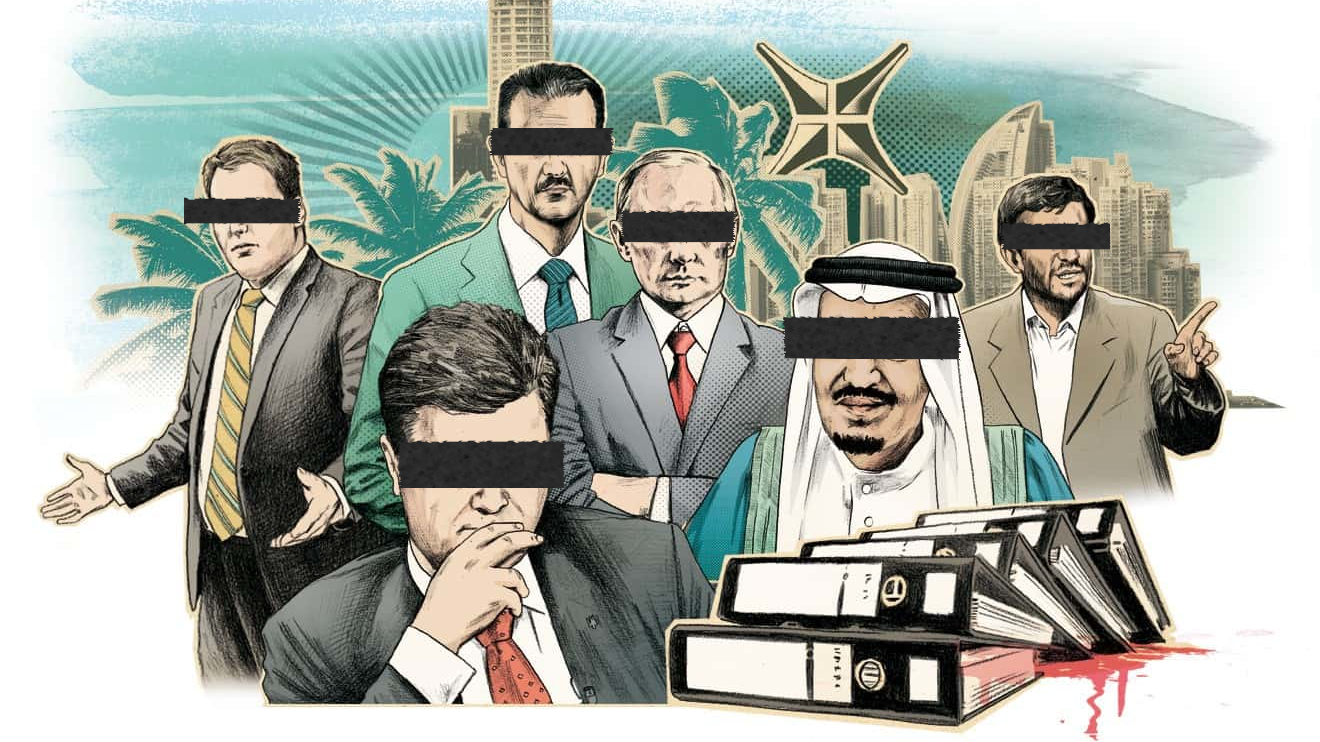
\includegraphics[
                        width = 1\paperwidth,
                        height = 1\paperheight,
                        keepaspectratio
                    ]{images/panamapapers/coverpanamapapershidden.jpg}
                };
            \end{pgfonlayer}
        \end{tikzpicture}
        \note[item]{
            Qualcuno saprebbe riconoscere chi sono le persone in questa slide?
        
            {\color{orange}\textit{wait 5 seconds}}
        }
        \note[item]{
            Vediamolo:
            
            {\color{blue}\textit{go to next slide}}
        }
    \end{frame}
    
    \begin{frame}{}
        \begin{tikzpicture}[remember picture,overlay]
            \begin{pgfonlayer}{background}
                \node[anchor=south east,outer sep=0pt,inner sep=0pt] at ($(current page.south east) +(-0in,0in)$) {
                    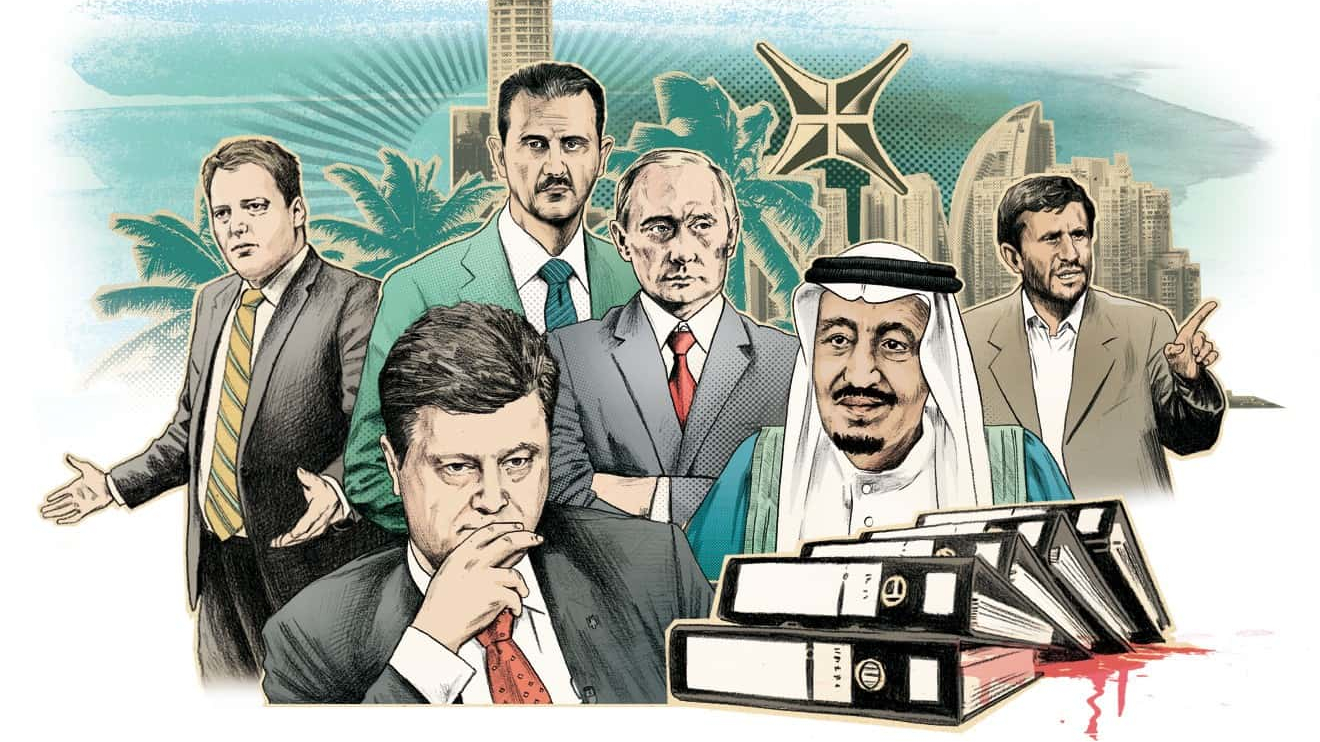
\includegraphics[
                        width = 1\paperwidth,
                        height = 1\paperheight,
                        keepaspectratio
                    ]{images/panamapapers/coverpanamapapersrevealed.jpg}
                };
            \end{pgfonlayer}
        \end{tikzpicture}
        \note[item]{
            Putin, Assad, Poroshenko, il re Salman, Ahmadinejad...
            
            Tutti politici di altissimo livello...
        }
        \note[item]{
            che apparvero nel...
            
            {\color{blue}\textit{go to next slide}}
        }
    \end{frame}
    
    \begin{frame}{}
        \begin{tikzpicture}[remember picture,overlay]
            \begin{pgfonlayer}{background}
                \node[anchor=south east,outer sep=0pt,inner sep=0pt] at ($(current page.south east) +(-0in,0in)$) {
                    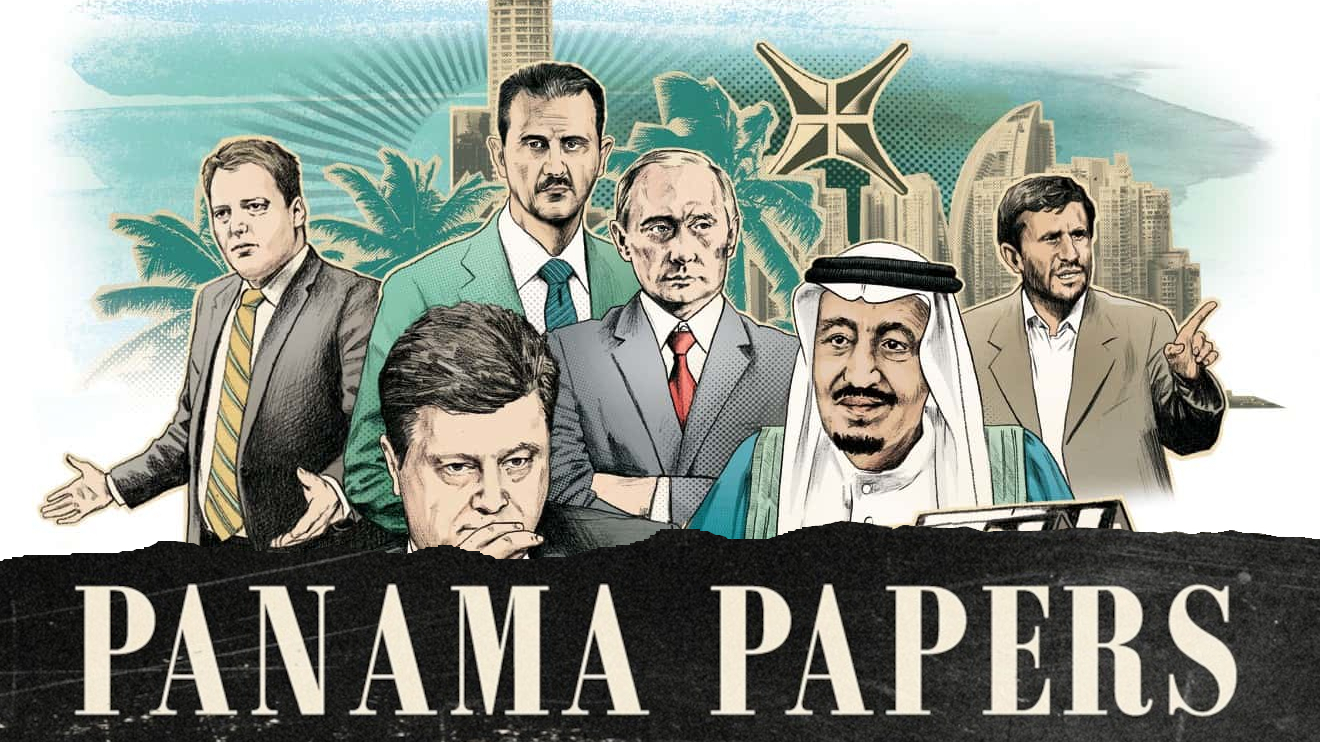
\includegraphics[
                        width = 1\paperwidth,
                        height = 1\paperheight,
                        keepaspectratio
                    ]{images/panamapapers/coverpanamapapersrevealedtitled.jpg}
                };
            \end{pgfonlayer}
        \end{tikzpicture}
        \note[item]{
            ...Panama Papers leak.
        }
        \note[item]{
            Ma cosa era Panama Papers?
            
            {\color{blue}\textit{go to next slide}}
        }
    \end{frame}
    
    \begin{frame}{}
        \begin{tikzpicture}[remember picture,overlay]
            \begin{pgfonlayer}{background}
                \node[anchor=south east,outer sep=0pt,inner sep=0pt] at ($(current page.south east) +(-0in,0in)$) {
                    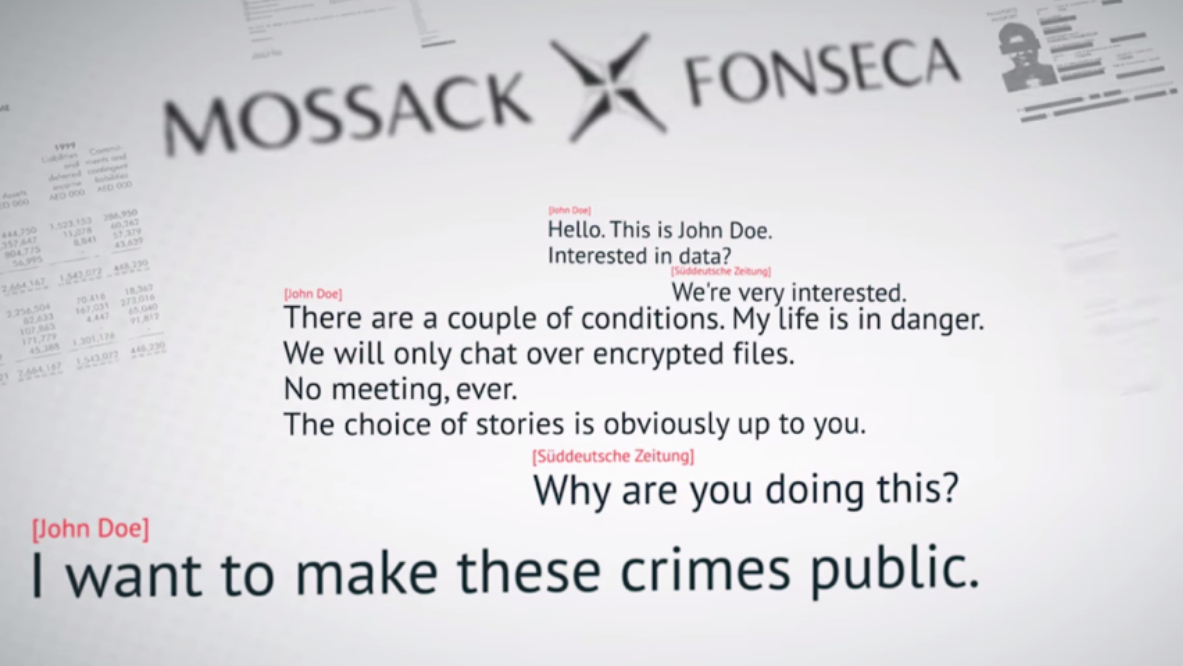
\includegraphics[
                        width = 1\paperwidth,
                        height = 1\paperheight,
                        keepaspectratio
                    ]{images/panamapapers/informer.jpg}
                };
            \end{pgfonlayer}
        \end{tikzpicture}
        \note[item]{
            \begin{itemize}
                \item In aprile 2016,
                \item grazie ad un informatore ...
            \end{itemize}
            
            {\color{blue}\textit{go to next slide}}
        }
    \end{frame}
    
    \begin{frame}{}
        \begin{tikzpicture}[remember picture,overlay]
            \begin{pgfonlayer}{background}
                \node[anchor=south east,outer sep=0pt,inner sep=0pt] at ($(current page.south east) +(-0in,0in)$) {
                    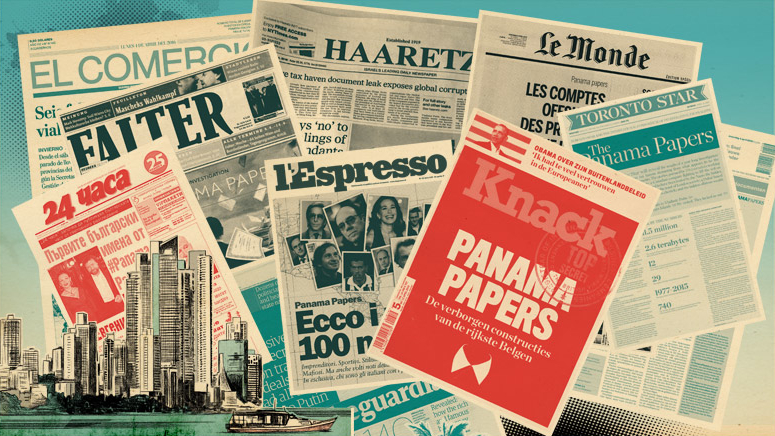
\includegraphics[
                        width = 1\paperwidth,
                        height = 1\paperheight,
                        keepaspectratio
                    ]{images/panamapapers/newspapers.jpg}
                };
            \end{pgfonlayer}
        \end{tikzpicture}
        \note[item]{
            \begin{itemize}
                \item ... l'inchiesta di 307 giornalisti da 76 paesi ha portato alla luce documenti e informazioni
                \item su migliardi di denaro dirottati da studi legali internazionali e banche verso paradisi fiscali
                \item per conto di...
            \end{itemize}
            
            {\color{blue}\textit{go to next slide}}
        }
    \end{frame}
    
    \begin{frame}{}
        \begin{tikzpicture}[remember picture,overlay]
            \begin{pgfonlayer}{background}
                \node[anchor=south east,outer sep=0pt,inner sep=0pt] at ($(current page.south east) +(-0in,0in)$) {
                    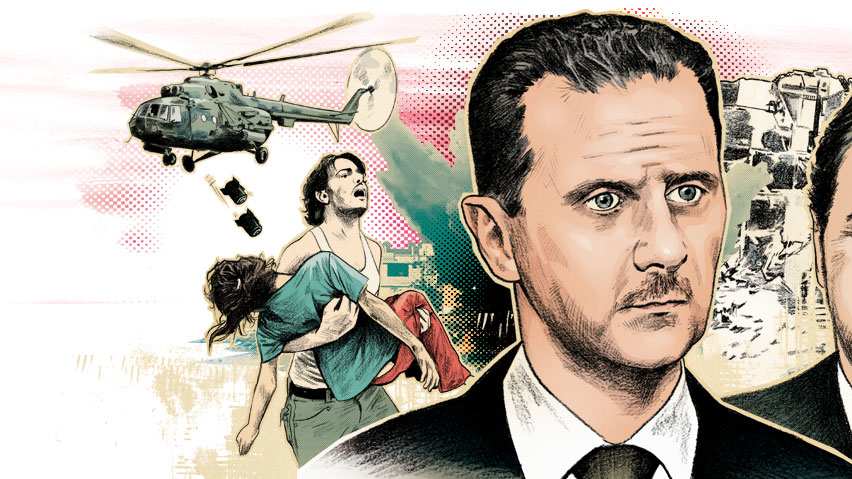
\includegraphics[
                        width = 1\paperwidth,
                        height = 1\paperheight,
                        keepaspectratio
                    ]{images/panamapapers/Assad.jpg}
                };
            \end{pgfonlayer}
        \end{tikzpicture}
        \note[item]{
            ... leader politici, criminali ...
            
            {\color{blue}\textit{go to next slide}}
        }
    \end{frame}
    
    \begin{frame}{}
        \begin{tikzpicture}[remember picture,overlay]
            \begin{pgfonlayer}{background}
                \node[anchor=south east,outer sep=0pt,inner sep=0pt] at ($(current page.south east) +(-0in,0in)$) {
                    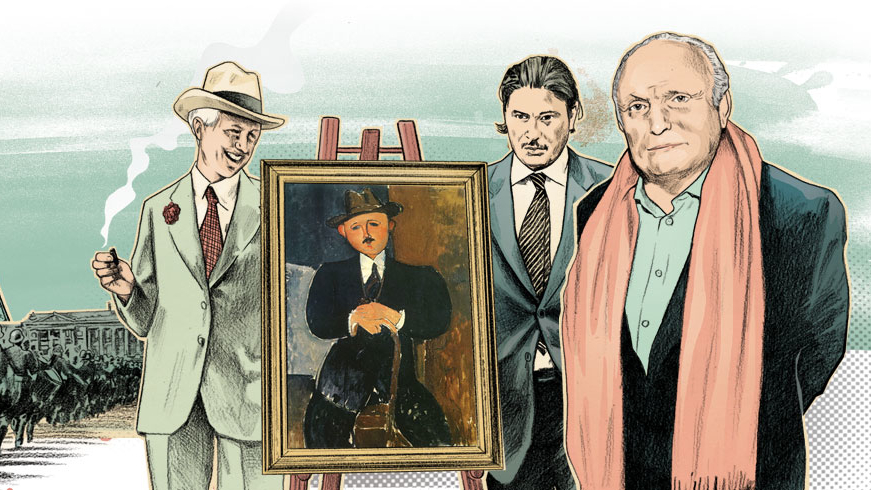
\includegraphics[
                        width = 1\paperwidth,
                        height = 1\paperheight,
                        keepaspectratio
                    ]{images/panamapapers/art.jpg}
                };
            \end{pgfonlayer}
        \end{tikzpicture}
        \note[item]{
            ... funzionari d'intelligence, artisti ...
            
            {\color{blue}\textit{go to next slide}}
        }
    \end{frame}
    
    \begin{frame}{}
        \begin{tikzpicture}[remember picture,overlay]
            \begin{pgfonlayer}{background}
                \node[anchor=south east,outer sep=0pt,inner sep=0pt] at ($(current page.south east) +(-0in,0in)$) {
                    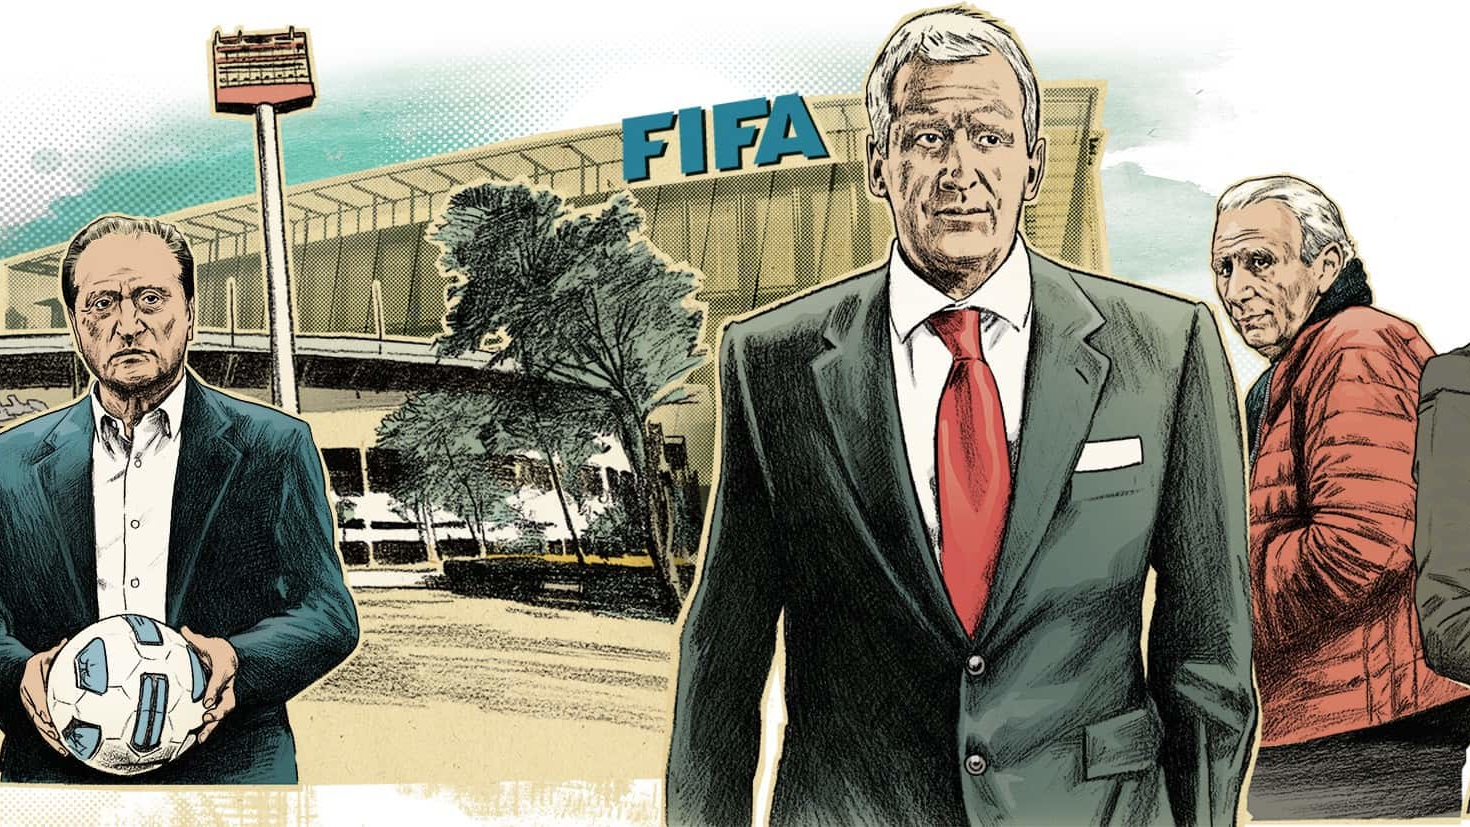
\includegraphics[
                        width = 1\paperwidth,
                        height = 1\paperheight,
                        keepaspectratio
                    ]{images/panamapapers/FIFA1.jpg}
                };
            \end{pgfonlayer}
        \end{tikzpicture}
        \note[item]{
            ... VIP dello sport ...
            
            {\color{blue}\textit{go to next slide}}
        }
    \end{frame}
    
    \begin{frame}{}
        \begin{tikzpicture}[remember picture,overlay]
            \begin{pgfonlayer}{background}
                \node[anchor=south east,outer sep=0pt,inner sep=0pt] at ($(current page.south east) +(-0in,0in)$) {
                    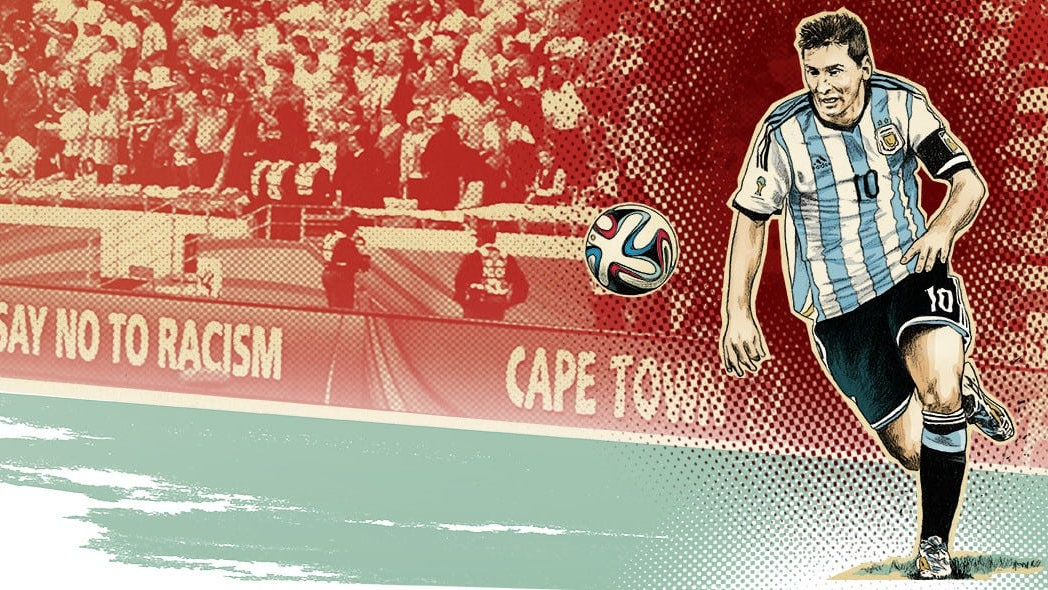
\includegraphics[
                        width = 1\paperwidth,
                        height = 1\paperheight,
                        keepaspectratio
                    ]{images/panamapapers/Messi.jpg}
                };
            \end{pgfonlayer}
        \end{tikzpicture}
        \note[item]{
            ... e dello spettacolo.
            
            {\color{orange}\textit{wait 5 seconds}}
        }
        \note[item]{
            \begin{itemize}
                \item Quanto era grande il dataset leakato?
                \item ... come erano strutturati i dati?
            \end{itemize}
            
            {\color{blue}\textit{go to next slide}}
        }
    \end{frame}
    
    \begin{frame}{}
        \begin{tikzpicture}[remember picture,overlay]
            \begin{pgfonlayer}{background}
                \node[anchor=south east,outer sep=0pt,inner sep=0pt] at ($(current page.south east) +(-0in,0in)$) {
                    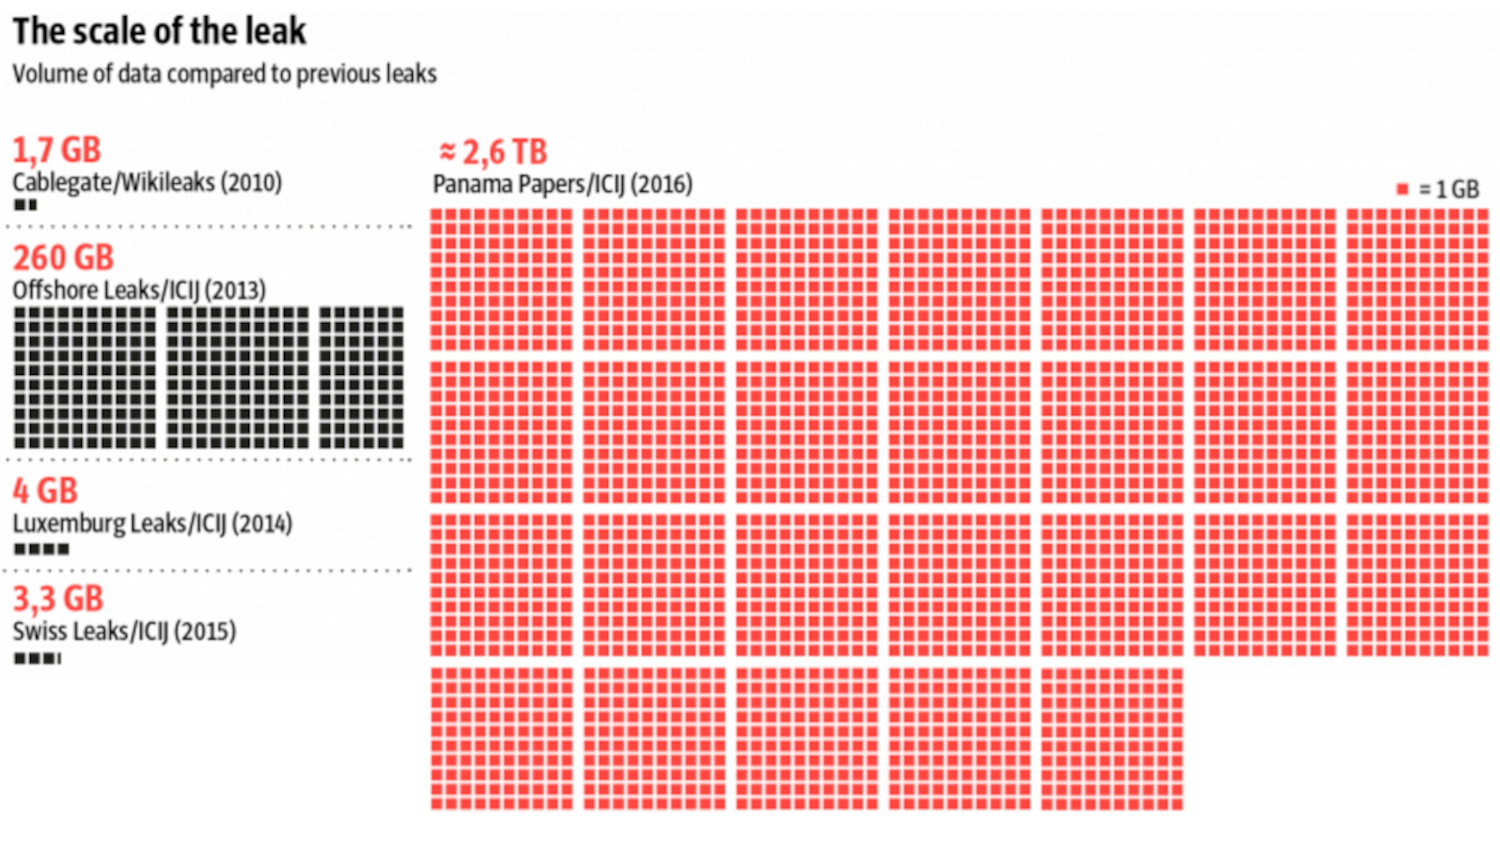
\includegraphics[
                        width = 1\paperwidth,
                        height = 1\paperheight,
                        keepaspectratio
                    ]{images/panamapapers/datasetsizenew.jpg}
                };
            \end{pgfonlayer}
        \end{tikzpicture}
        \note[item]{
            Il leak era di dimensione 2.6 TB, 1500 volte più grande del Cablegate del 2010 di Wikileaks.
            
            {\color{blue}\textit{go to next slide}}
        }
    \end{frame}
    
    \begin{frame}{}
        \begin{tikzpicture}[remember picture,overlay]
            \begin{pgfonlayer}{background}
                \node[anchor=south east,outer sep=0pt,inner sep=0pt] at ($(current page.south east) +(-0in,0in)$) {
                    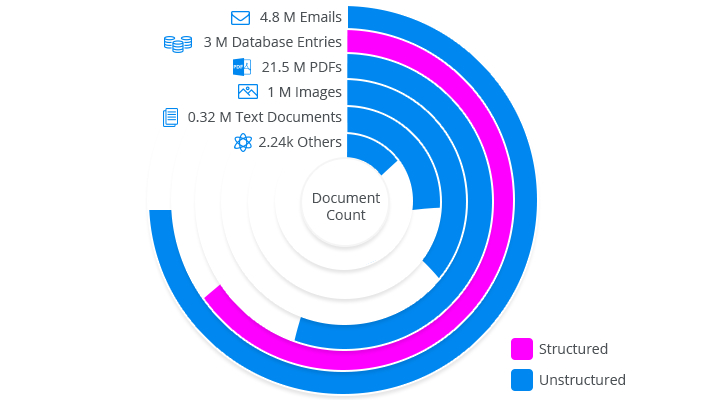
\includegraphics[
                        width = 1\paperwidth,
                        height = 1\paperheight,
                        keepaspectratio
                    ]{images/panamapapers/datatypes.jpg}
                };
            \end{pgfonlayer}
        \end{tikzpicture}
        \note[item]{
            La maggior parte dei dati erano non strutturati, sotto forma di emails, immagini e files PDF inviati.
            
            {\color{blue}\textit{go to next slide}}
        }
    \end{frame}
    
    \begin{frame}{}
        \begin{tikzpicture}[remember picture,overlay]
            \begin{pgfonlayer}{background}
                \node[anchor=south east,outer sep=0pt,inner sep=0pt] at ($(current page.south east) +(-0in,0in)$) {
                    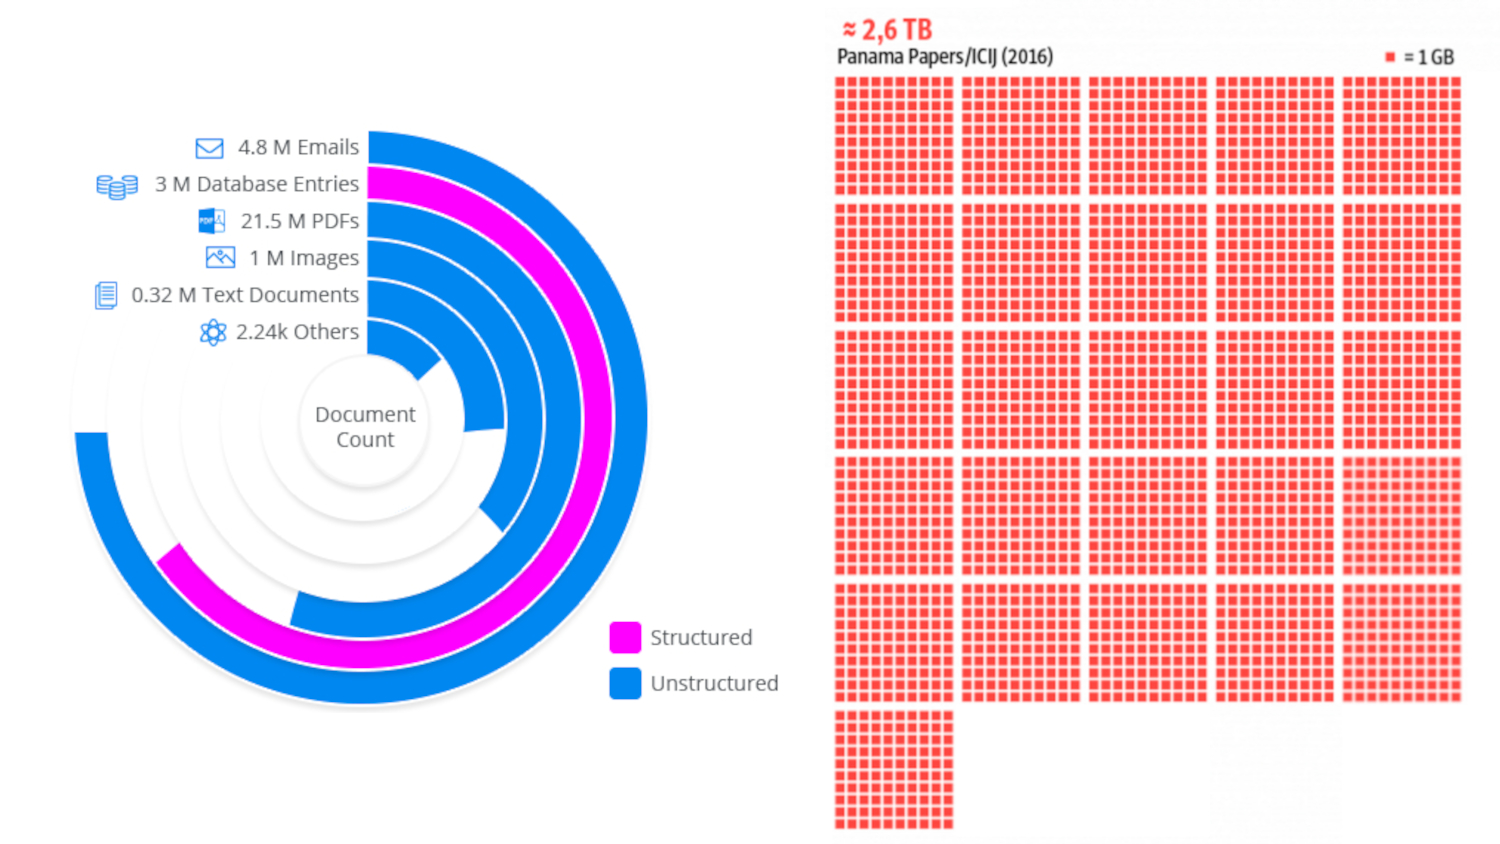
\includegraphics[
                        width = 1\paperwidth,
                        height = 1\paperheight,
                        keepaspectratio
                    ]{images/panamapapers/datasetsizeandtypes.jpg}
                };
            \end{pgfonlayer}
        \end{tikzpicture}
        \note[item]{
            \begin{itemize}
                \item Una domanda sorge spontanea:
                \item Come si può indagare su un dataset così immenso
                \item e in gran parte fatto di dati non strutturati?
            \end{itemize}
            
            {\color{blue}\textit{go to next slide}}
        }
    \end{frame}
    
    \begin{frame}{}
        \begin{tikzpicture}[remember picture,overlay]
            \begin{pgfonlayer}{background}
                \node[anchor=south east,outer sep=0pt,inner sep=0pt] at ($(current page.south east) +(-0in,0in)$) {
                    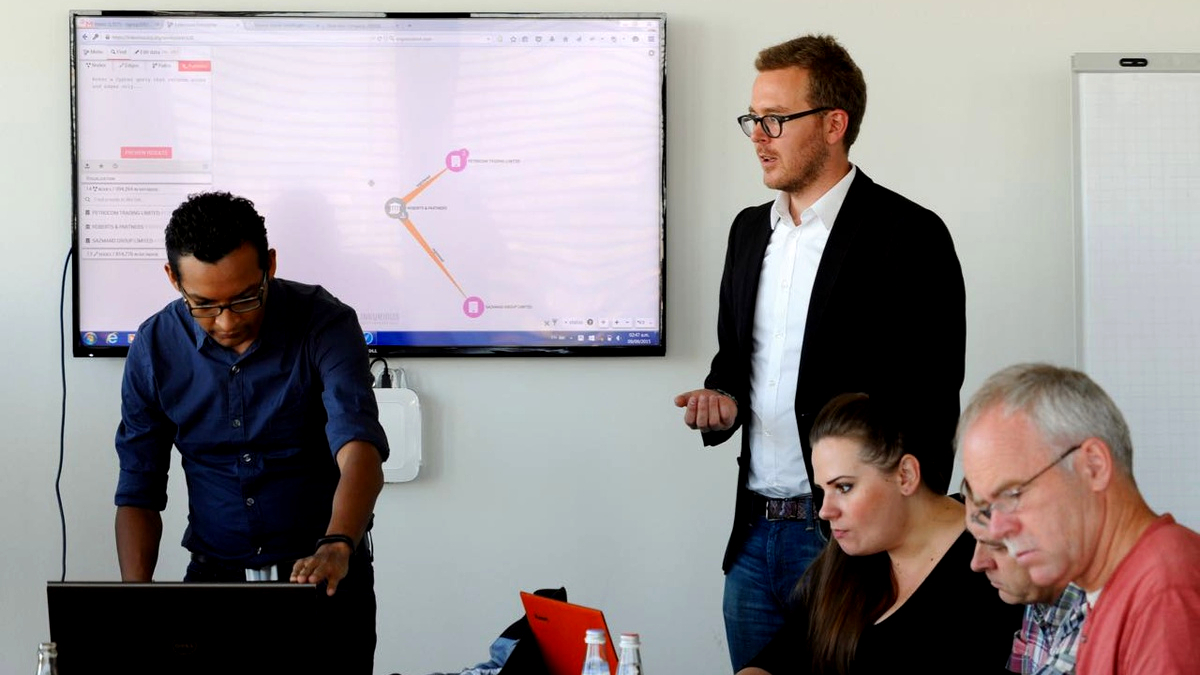
\includegraphics[
                        width = 1\paperwidth,
                        height = 1\paperheight,
                        keepaspectratio
                    ]{images/panamapapers/team.jpg}
                };
            \end{pgfonlayer}
        \end{tikzpicture}
        \note[item]{
            Loro, un team composto da giornalisti investigativi ed esperti di database a grafi ce l'hanno fatta.
            
            {\color{blue}\textit{go to next slide}}
        }
    \end{frame}
    
    \begin{frame}{}
        \begin{tikzpicture}[remember picture,overlay]
            \begin{pgfonlayer}{background}
                \node[anchor=south east,outer sep=0pt,inner sep=0pt] at ($(current page.south east) +(-0in,0in)$) {
                    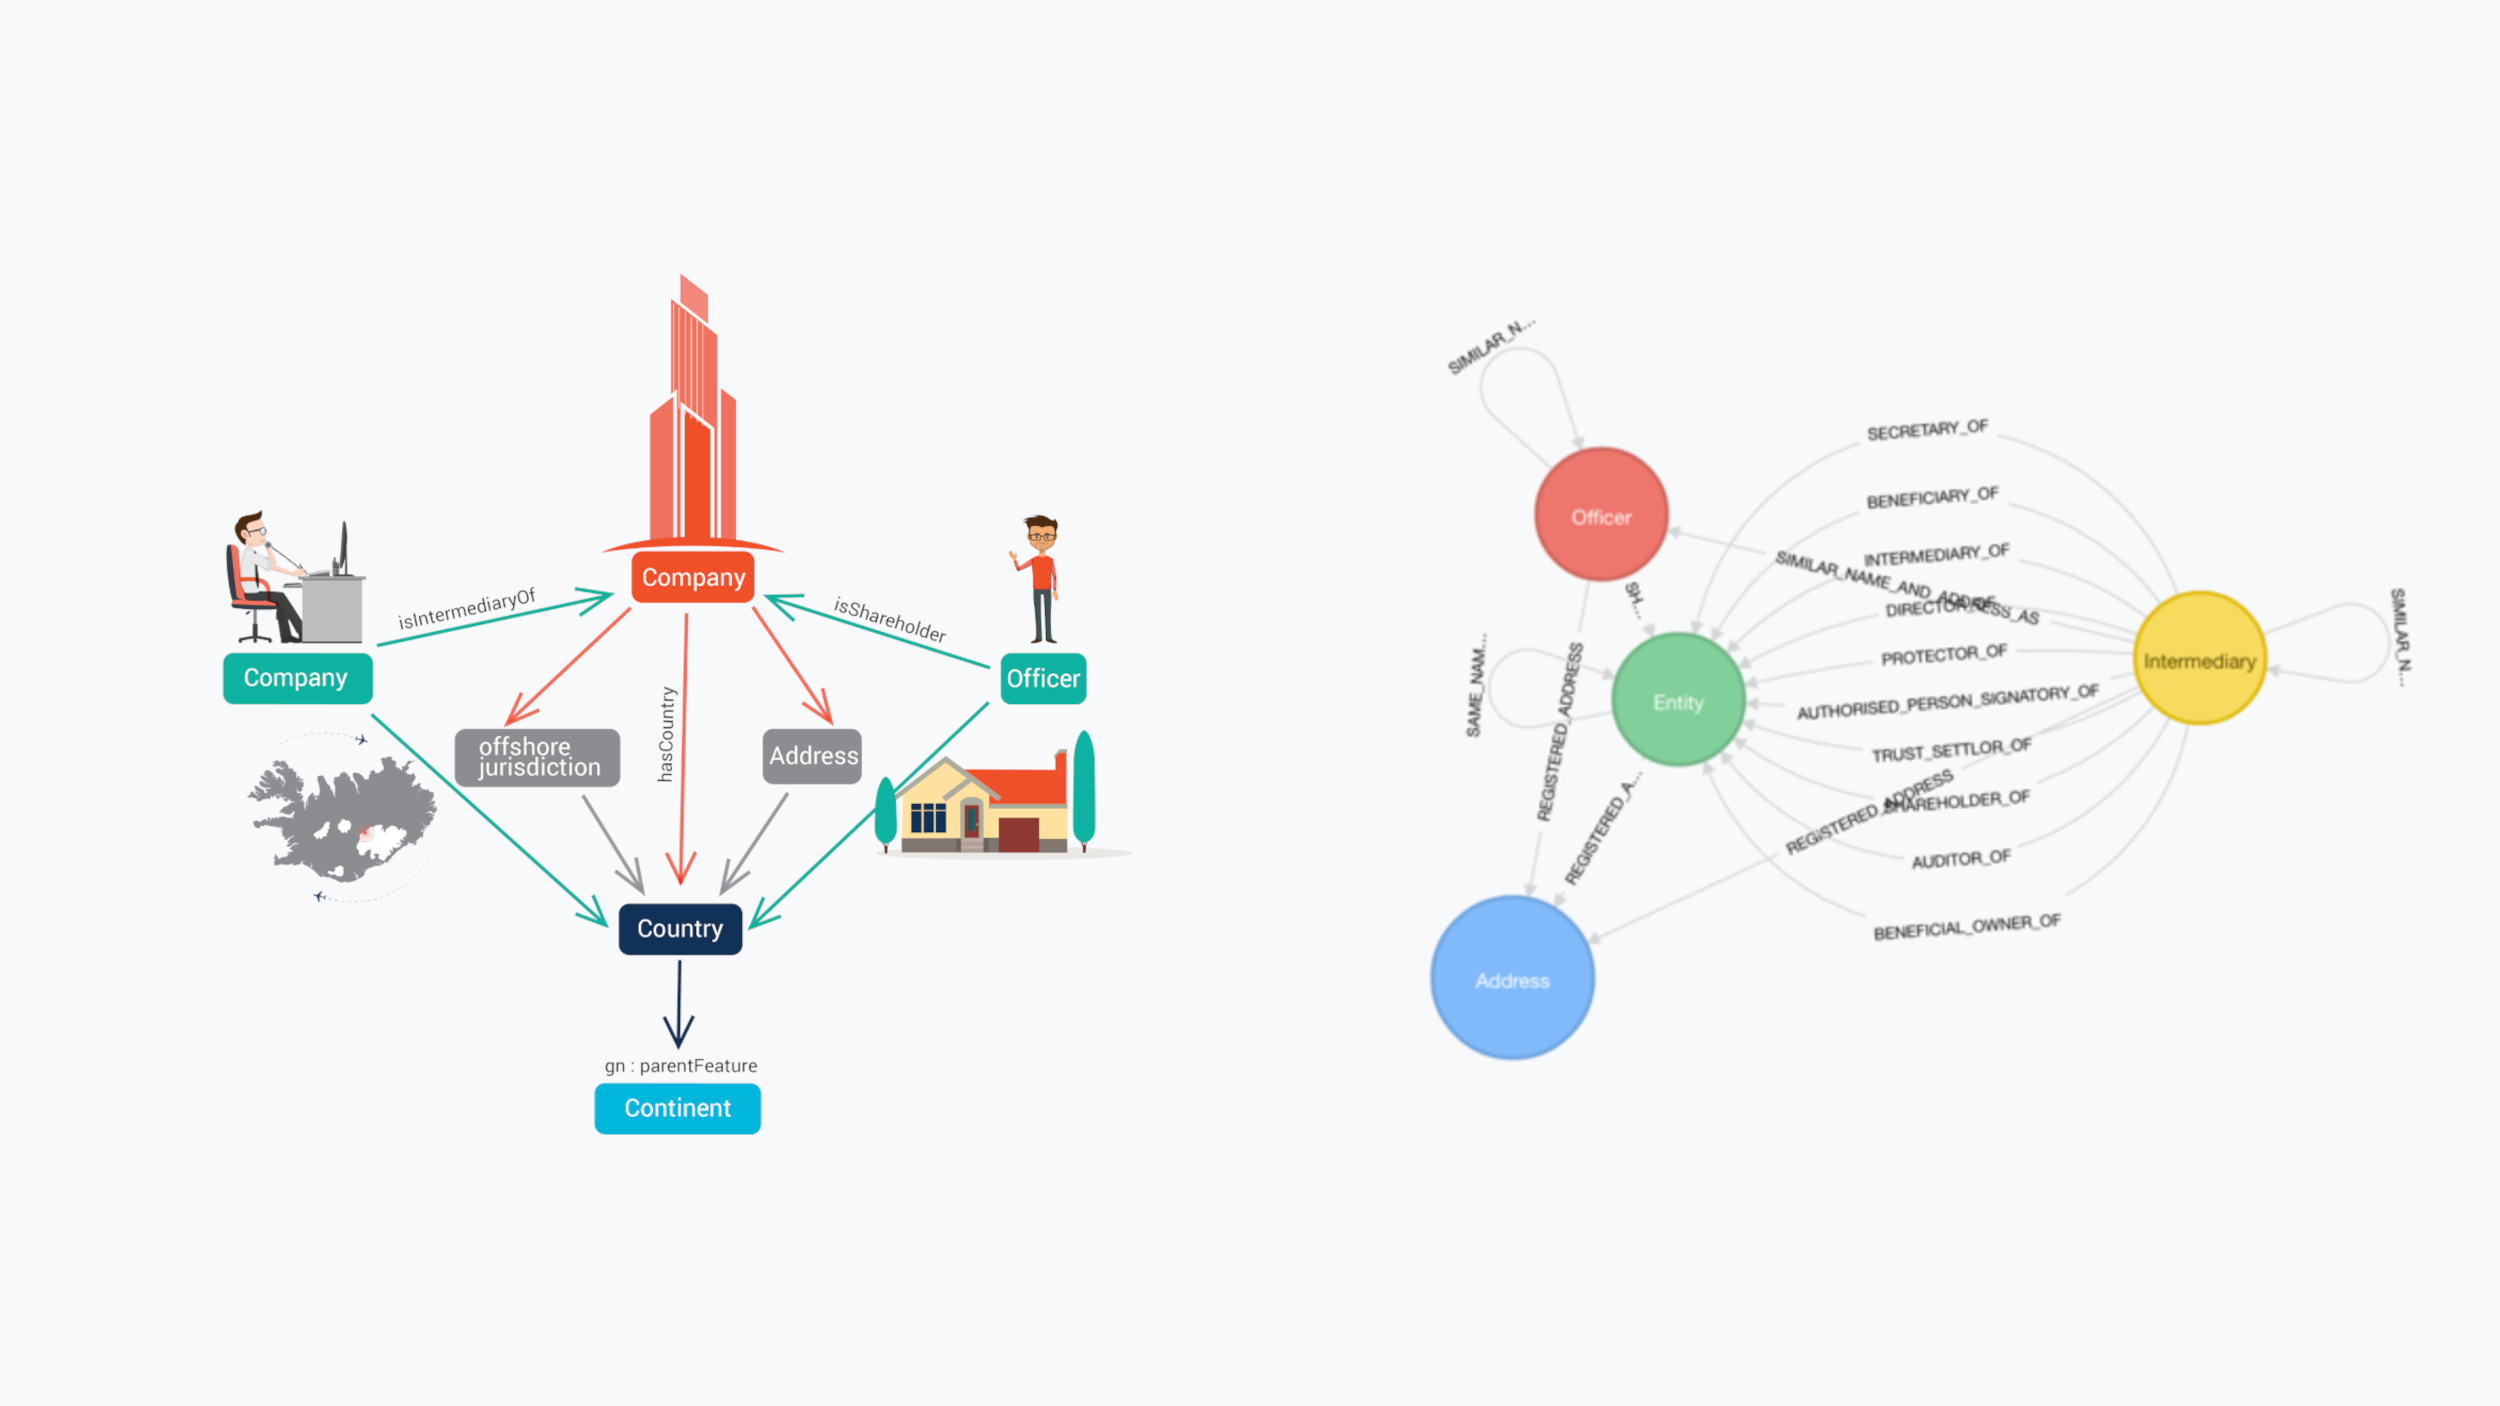
\includegraphics[
                        width = 1\paperwidth,
                        height = 1\paperheight,
                        keepaspectratio
                    ]{images/panamapapers/graphsmall.jpg}
                };
            \end{pgfonlayer}
        \end{tikzpicture}
        \note[item]{
            Facendo buon uso delle relazioni che derivano da dati interconnessi (ad esempio le mail, le dipendenze tra le entità) ...
            
            {\color{blue}\textit{go to next slide}}
        }
    \end{frame}
    
    \begin{frame}{}
        \begin{tikzpicture}[remember picture,overlay]
            \begin{pgfonlayer}{background}
                \node[anchor=south east,outer sep=0pt,inner sep=0pt] at ($(current page.south east) +(-0in,0in)$) {
                    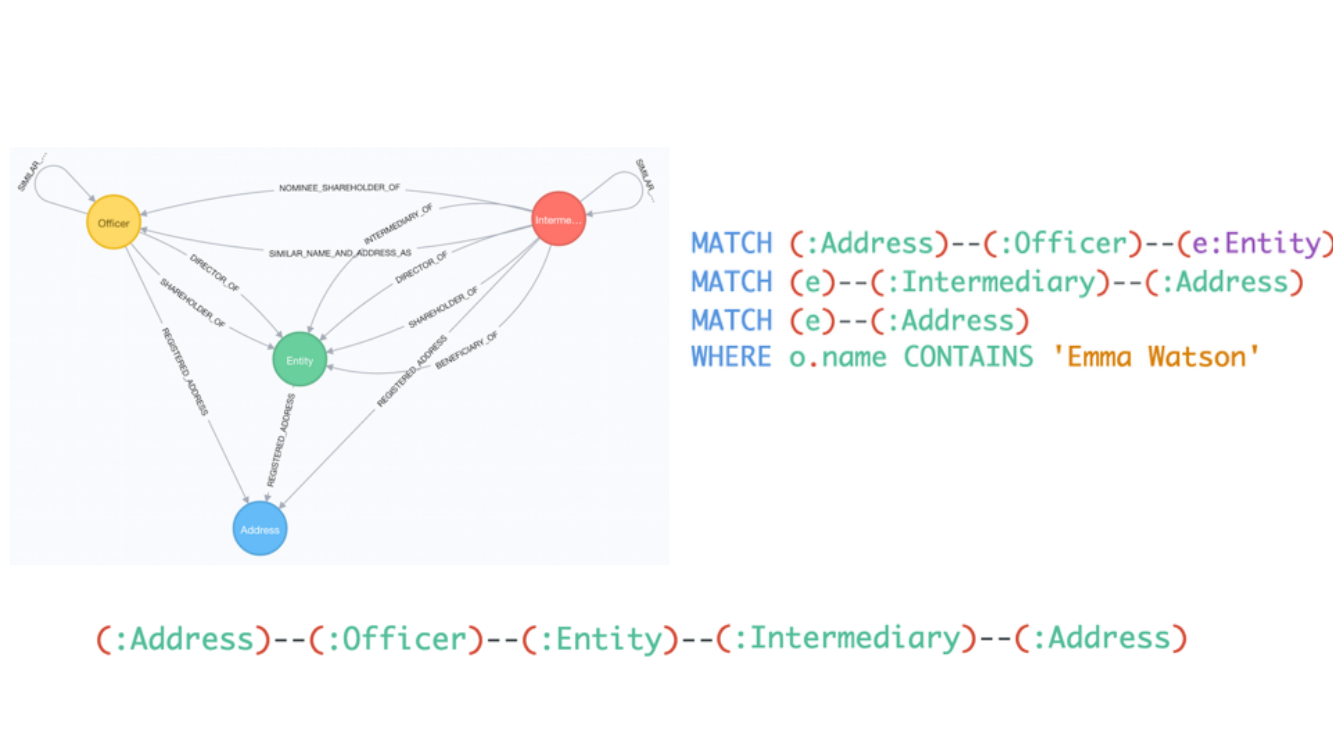
\includegraphics[
                        width = 1\paperwidth,
                        height = 1\paperheight,
                        keepaspectratio
                    ]{images/panamapapers/neo4jcypher.jpg}
                };
            \end{pgfonlayer}
        \end{tikzpicture}
        \note[item]{
            \begin{itemize}
                \item ... e di nuove tecnologie (come i database a grafi),
                \item hanno generato grafi con nodi rappresentanti le entità coinvolte
                \item e archi rappresentanti le connessioni tra loro,
            \end{itemize}
            
            {\color{blue}\textit{go to next slide}}
        }
    \end{frame}
    
    \begin{frame}{}
        \begin{tikzpicture}[remember picture,overlay]
            \begin{pgfonlayer}{background}
                \node[anchor=south east,outer sep=0pt,inner sep=0pt] at ($(current page.south east) +(-0in,0in)$) {
                    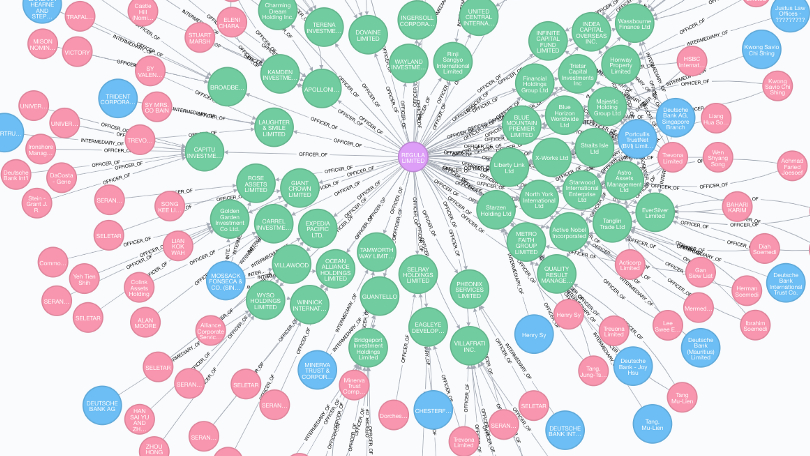
\includegraphics[
                        width = 1\paperwidth,
                        height = 1\paperheight,
                        keepaspectratio
                    ]{images/panamapapers/graph.jpg}
                };
            \end{pgfonlayer}
        \end{tikzpicture}
        \note[item]{
            \begin{itemize}
                \item il tutto interrogabile
            \end{itemize}
        }
        \note[item]{
            \begin{itemize}
                \item Questo è uno dei più eclatanti esempi a queste dimensioni
                \item dell'utilizzo di database a grafi per svolgere un compito
                \item che altri tipi di database semplicemente non potevano fare
                \item (almeno i tempi di interrogazione non sarebbero stati umanamente accettabili)
                \item perché non progettati per effettuare visite su grafi con dati non strutturati.
            \end{itemize}
        }
        \note[item]{
            \begin{itemize}
                \item Nel lavoro svolto per la tesi, non si è parlato di Panama Papers.
                \item Ma:
            \end{itemize}
            
            {\color{blue}\textit{go to next slide}}
        }
    \end{frame}
    
    \begin{frame}[noframenumbering, standout]
        \normalfont
        
        \vspace*{0.75cm}
        \fontsize{26pt}{33pt}\selectfont\textsc{\break\mydocumenttitle}
        
        \begin{columns}[t]
            \column{0.13\textwidth}
            
            \column{0.69\textwidth}
                \vspace*{-1.25cm}
                \begin{center}
                    \Large\normalfont\mydocumentsubtitle
                    
                    \vspace*{0.5cm}
                    \normalsize\textbf{\myauthor}
                \end{center}
                
                    
                %\mydateofpublishing
                
                \begin{tikzpicture}[remember picture,overlay]
                    \begin{pgfonlayer}{background}
                        \node[anchor=south east,outer sep=0pt,inner sep=0pt] at ($(current page.south east) +(-0in,0in)$) {
                            
\includegraphics[
                                width = 0.25\paperwidth
                            ]{images/LogoUniBGwhiterotatedcut.pdf}
                        };
                    \end{pgfonlayer}
                \end{tikzpicture}
                
            \column{0.13\textwidth}
        \end{columns}
        \note[item]{
            \normalfont
            \begin{itemize}
                \item Facendo uso di un database a grafi per il salvataggio
                \item e l'interrogazione di dati di un dataset di 5.6 milioni di pubblicazioni scientifiche accademiche da 2.8 milioni di ricercatori,
                \item applicando al grafo da essi generati un algoritmo di Community Detection,
                \item ovvero, di individuazione delle communità
                \item sono state individuate 180 mila Communities.
                \item Inoltre, è stata sviluppata una Full-Stack Web Application per visualizzare queste communità di collaborazione.
            \end{itemize}
        }
        \note[item]{
            \normalfont
            Più in dettaglio:
            
            {\color{blue}\textit{go to next slide}}
        }
    \end{frame}
    
    \begin{frame}{The work done}
        \begin{enumerate}
            \item \textbf{Literature review} of graph theory, graph databases and clustering algorithms.
            \item \texttt{dblp.org} \textbf{Dataset download, conversion \& import} in ArangoDB Graph DBMS.
            \item \textbf{Data transformations} to obtain vertices, edges and the complete graph.
            \item \textbf{Community Detection Algorithm application} on the graph for clustering.
            \item \textbf{Web Application development} to display the results of the clustering.
        \end{enumerate}
        
        \note[item]{
            \begin{itemize}
                \item \footnotesize È stata fatta una consultazione in letteratura dei concetti base di teoria dei grafi,
                \item \footnotesize delle varie caratteristiche dei database a grafi
                \item \footnotesize e degli algoritmi per l'individuazione delle communities in grafi.
            \end{itemize}
        }
        \note[item]{
            \begin{itemize}
                \item \footnotesize Poi è stato scaricato il dataset da dblp.org, è stato convertito
                \item \footnotesize e importato su ArangoDB, il graph database management system scelto.
            \end{itemize}
        }
        \note[item]{
            \begin{itemize}
                \item \footnotesize Le collezioni di dati sono state sottoposte a trasformazioni per ottenere vertici,
                \item \footnotesize archi e da questi il grafo completo dell'intero dataset.
            \end{itemize}
        }
        \note[item]{
            \begin{itemize}
                \item \footnotesize Su tale grafo poi è stato applicato un Label Propagation Community Detection Algorithm,
                \item \footnotesize ovvero un algoritmo a propagazione di etichette per l'individuazione delle communità di collaborazione scientifica.
            \end{itemize}
        }
        \note[item]{
            \begin{itemize}
                \item \footnotesize In fine, è stata sviluppata una Web Application per visualizzare le communities individuate.
            \end{itemize}
        }
        \note[item]{
            \footnotesize Vediamoli uno ad uno...
            
            \large {\color{blue}\textit{go to next slide}}
        }
    \end{frame}
    
    \begin{frame}{Graph databases}
        \centering
        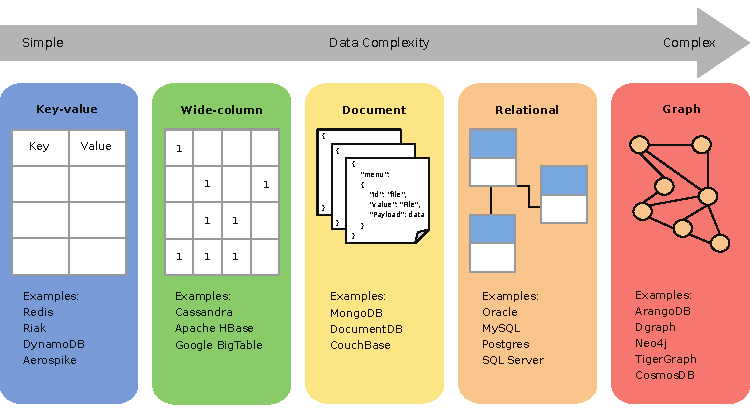
\includegraphics[width = 0.78\paperwidth, height = 0.78\paperheight, keepaspectratio]{images/BechbergerPerryman2020page8.pdf}
        
        \note[item]{
            \begin{itemize}
                \item ... più i dati sono interconnessi e strutturati in modo complesso,
                \item più fa senso usare database a grafi
            \end{itemize}
        }
        \note[item]{
            \begin{itemize}
                \item Inoltre se i nested JOINs da fare durante un'interrogazione sono più di 3 livelli di profondità,
            \end{itemize}
            
            {\color{blue}\textit{go to next slide}}
        }
    \end{frame}
    
    \begin{frame}{}
        \begin{tikzpicture}[remember picture,overlay]
            \begin{pgfonlayer}{background}
                \node[anchor=south east,outer sep=0pt,inner sep=0pt] at ($(current page.south east) +(-0in,0in)$) {
                    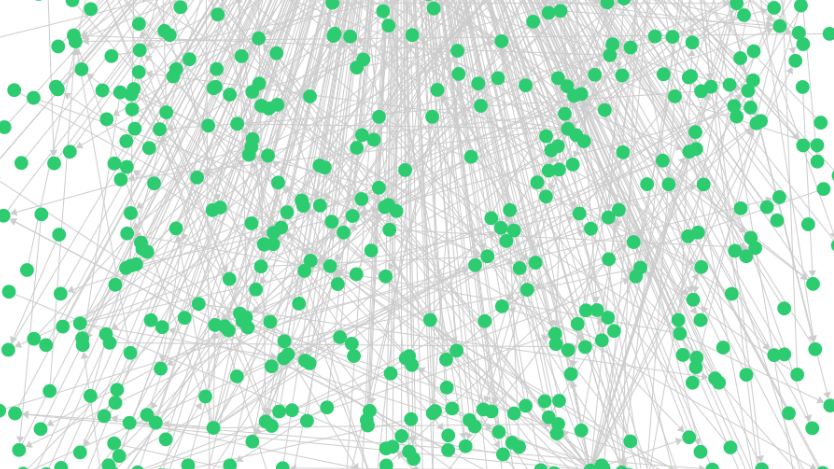
\includegraphics[
                        width = 1\paperwidth,
                        height = 1\paperheight,
                        keepaspectratio
                    ]{images/PregelDetectedCommunityOtherVerticesResultcut.jpg}
                };
            \end{pgfonlayer}
        \end{tikzpicture}
        \note[item]{
            \begin{itemize}
                \item ovverò, in termini di grafi, se bisogna fare più di 3 salti di attraversamento degli archi,
                \item allora i tempi di interrogazione usando database tradizionali diventano proibitivi.
            \end{itemize}
        }
        \note[item]{
            \begin{itemize}
                \item Dunque, vediamo ora concretamente cosa è stato fatto.
            \end{itemize}
            
            {\color{blue}\textit{go to next slide}}
        }
    \end{frame}
    
    \begin{frame}{Le macchine}
        \begin{tikzpicture}[remember picture,overlay]
            \begin{pgfonlayer}{background}
                \node[anchor=south east,outer sep=0pt,inner sep=0pt] at ($(current page.south east) +(-0in,0in)$) {
                    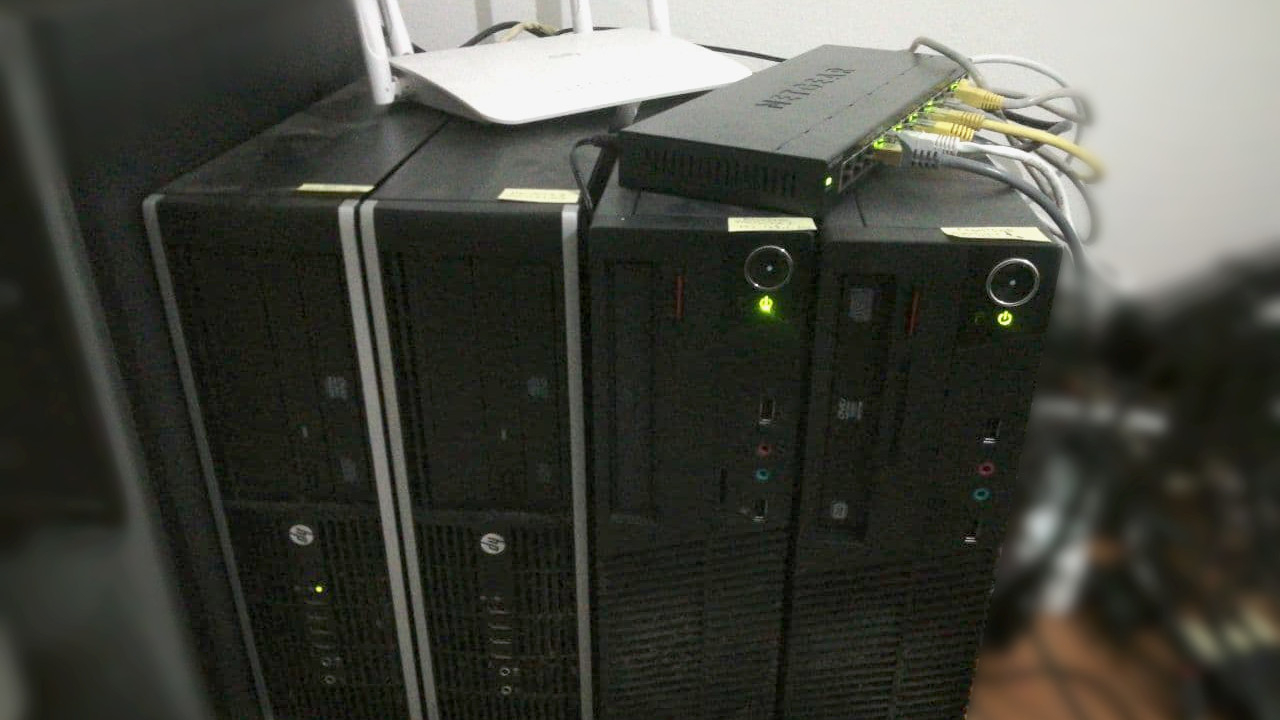
\includegraphics[
                        width = 1\paperwidth,
                        height = 1\paperheight,
                        keepaspectratio
                    ]{images/machinesphotocut.jpg}
                };
            \end{pgfonlayer}
        \end{tikzpicture}
        \note[item]{
            \begin{itemize}
                \item Al fine di hostare il database,
                \item servire l'API della Web Application
                \item e l'interfaccia lato frontend del sito,
                \item 3 macchine separate, un router e uno switch sono stati usati.
                \item La quarta macchina è stata usata a scopi di sviluppo e accesso remoto.
            \end{itemize}
        }
        \note[item]{
            \begin{itemize}
                \item Una volta installato i sistemi operativi e ArangoDB sula macchina scelta come host del database...
            \end{itemize}
            
            {\color{blue}\textit{go to next slide}}
        }
    \end{frame}
    
    \begin{frame}{The dataset: dblp.org}
        \begin{center}
            \vspace*{-0.1cm}
            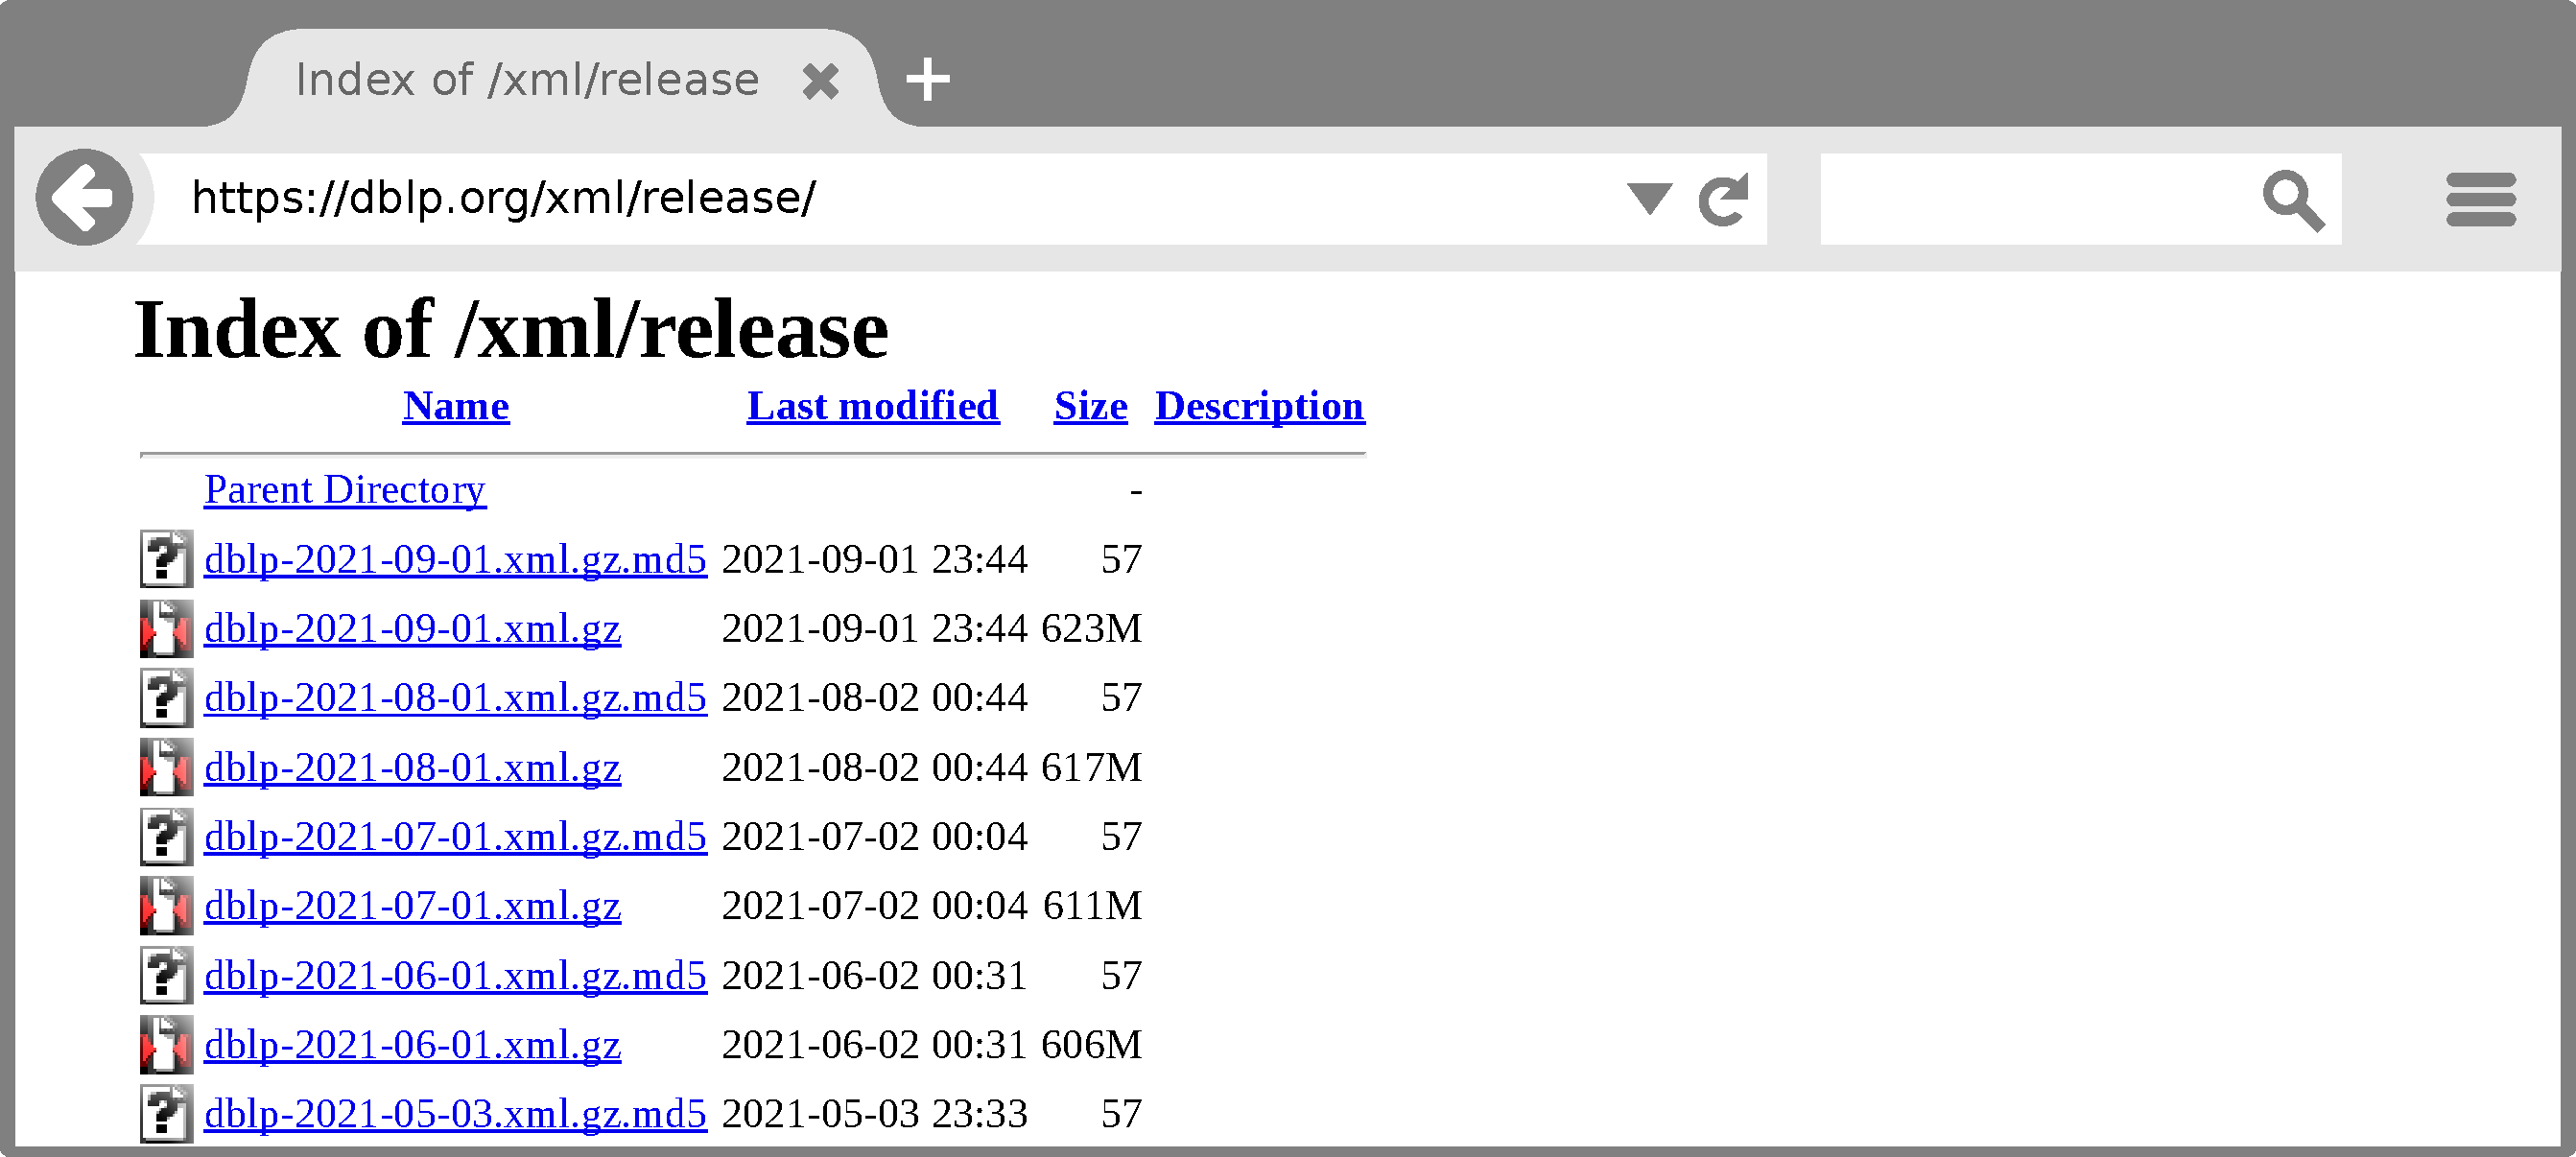
\includegraphics[
                width = 0.70\paperwidth,
                height = 0.70\paperheight,
                keepaspectratio
            ]{images/dblpdatasetdownload.pdf}
        \end{center}
        
        \vspace*{-0.3cm}
        {\color{darkgray}The dataset:}
        \begin{columns}[t]
            \column{.50\textwidth}
                \vspace*{-0.6cm}
                \begin{itemize}
                	\item Compressed archive of 623 MB.
                	\item Once decompressed: Single XML file of 3.2 GB.
                \end{itemize}
                
            \column{.50\textwidth}
                \vspace*{-0.6cm}
                \begin{itemize}
                	\item 8.5 million XML entries on publications, authors, journals, institutions, citations etc.
                \end{itemize}
        \end{columns}
        \note[item]{
            {\color{blue}\textit{go to next slide}}
        }
    \end{frame}
    
    \begin{frame}{Data conversion, import and transformations}
        \begin{center}
            \vspace*{-0.1cm}
            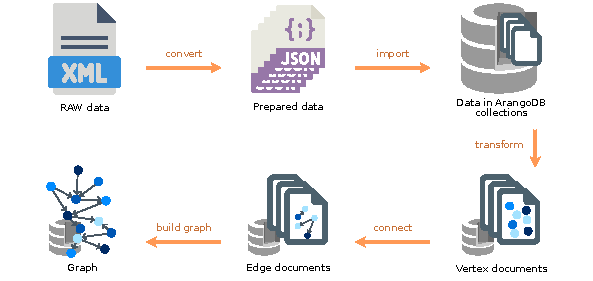
\includegraphics[
                width = 0.7\paperwidth,
                height = 0.7\paperheight,
                keepaspectratio
            ]{images/datatransformations.pdf}
        \end{center}
        
        \vspace*{-0.3cm}
        {\color{darkgray}The steps:}
        \begin{columns}[t]
            \column{.50\textwidth}
                \vspace*{-0.3cm}
                \begin{enumerate}
                	\item \small Conversion from XML to line JSON;
                	\item \small Import in ArangoDB collection;
                \end{enumerate}
                
            \column{.50\textwidth}
                \vspace*{-1.3cm}
                \begin{enumerate}
                    \setcounter{enumi}{2}
                	\item \small Transform imported data to vertex documents;
                	\item \small Link vertices by edges;
                	\item \small Build the graph.
                \end{enumerate}
        \end{columns}
        \note[item]{
            {\color{blue}\textit{go to next slide}}
        }
    \end{frame}
    
    \begin{frame}{The graph}
        
        \begin{columns}
            \column{.30\textwidth}
                \small
                {\color{darkgray}A subgraph of the obtained final graph:}
            
            \column{.70\textwidth}
                \begin{center}
                    \vspace*{-0.2cm}
                    \hspace*{0.1cm}
                    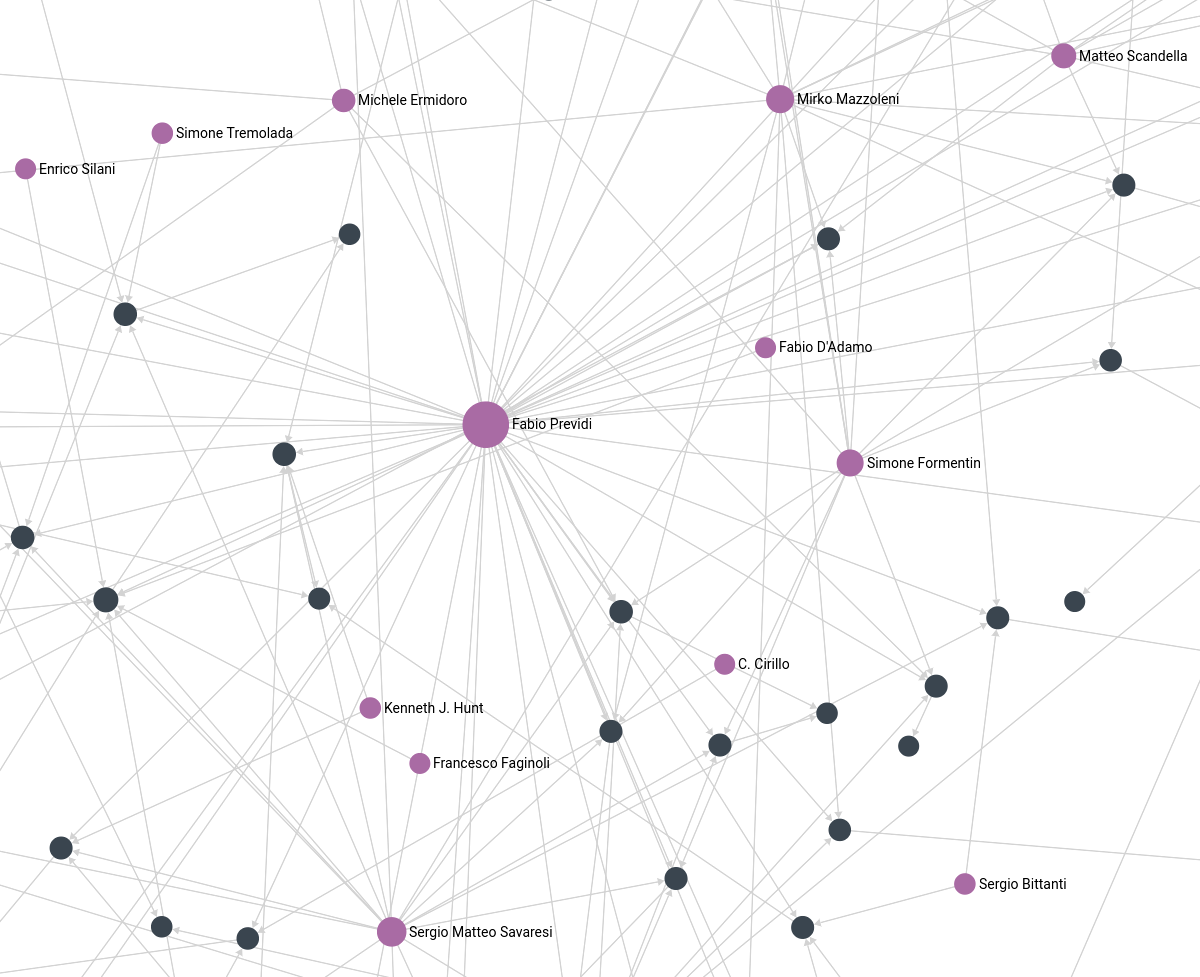
\includegraphics[
                        width = 1\textwidth,
                        height = 0.85\paperheight,
                        keepaspectratio
                    ]{images/SnapshotArangoDBGraphPrevidiMazzolenishort.png}
                \end{center}
        \end{columns}
        \note[item]{
            Questo è un assaggio del grafo finale, o anche una verifica della sua validità.
        }
        \note[item]{
            Il grafo finale è composto dall'insieme di tutti i vertici del dataset e da tutte le connessioni derivanti dalle informazioni dei loro attributi.
        }
        \note[item]{
            In questo sottografo sono mostrate le connessioni di primo e secondo grado del professor Previdi, il vertice in mezzo.
        }
        \note[item]{
            Si può notare in alto a destra professor Mazzoleni e Scandella.
        }
        \note[item]{
            In alto a sinistra professor Ermidoro e in basso a destra professor Bitanti.
            
            {\color{blue}\textit{go to next slide}}
        }
    \end{frame}
    
    \begin{frame}{Pregel Label Propagation Community Detection Algorithm}
        \begin{center}
            \vspace*{-0.1cm}
            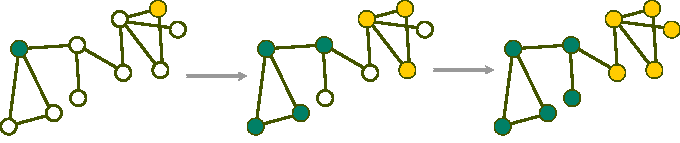
\includegraphics[
                width = 0.85\paperwidth,
                height = 0.85\paperheight,
                keepaspectratio
            ]{images/labelpropagation.pdf}
        \end{center}
        
        \vspace*{-0.3cm}
        {\color{darkgray}The algorithm:}
        \begin{columns}[t]
            \column{.50\textwidth}
                \vspace*{-0.4cm}
                \begin{enumerate}
                	\item \small Every vertex is labeled with a unique label.
                	\item \small The labels are propagated from vertex to vertex.
                	\item \small At the end of an iteration, each vertex updates its label to the one with maximum weight of neighbor vertices.
                \end{enumerate}
                
            \column{.50\textwidth}
                \vspace*{-0.7cm}
                \begin{enumerate}
                    \setcounter{enumi}{3}
                	\item \small Convergence is reached when each vertex is labeled as the majority of its neighbors.
                	It may happen that convergence is not reached in a reasonable time.
                	In such cases, setting a maximum number of iterations would be a trade-off between accuracy and execution time.
                \end{enumerate}
        \end{columns}
        \note[item]{
            Every vertex is labeled with a unique label.
        }
        \note[item]{
            The labels are propagated from vertex to vertex throughout the graph.
        }
        \note[item]{
            At the end of each propagation iteration, each vertex updates its label to match the one with the maximum weight, which is calculated based on the weights of neighbor vertices and their relationships.
            Ties are broken uniformly and randomly.
        }
        \note[item]{
            Convergence is reached when each vertex is labeled as the majority of its neighbors.
            It may happen that convergence on a single solution is not reached in a reasonable time. In such cases, a trade-off between accuracy and execution time would be setting a maximum number of iterations to avoid maybe never-ending execution.
            
            {\color{blue}\textit{go to next slide}}
        }
    \end{frame}
    
    \begin{frame}{A generic Pregel algorithm}
        
        \hspace*{-0.7cm}
        {\color{darkgray}Pregel's supersteps:}
        \begin{columns}[t]
            \column{.35\textwidth}
                \vspace*{-0.3cm}
                
                \hspace*{-0.1cm}
                \small \textbf{Diffusion}: information is propagated from vertex to neighbors
                
                \hspace*{-0.1cm}
                \small \textbf{Fusion}: information is aggregated from neighbors to a set of entities
                
            \column{.65\textwidth}
                \vspace*{-1cm}
                \hspace*{-2cm}
                \begin{center}
                    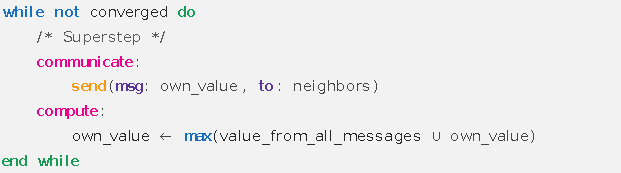
\includegraphics[
                        width = 0.6\paperwidth,
                        height = 0.6\paperheight,
                        keepaspectratio
                    ]{images/pregelpseudocode.pdf}
                \end{center}
                
                \vspace*{-0.1cm}
                \begin{center}
                    \hspace*{-4.7cm}
                    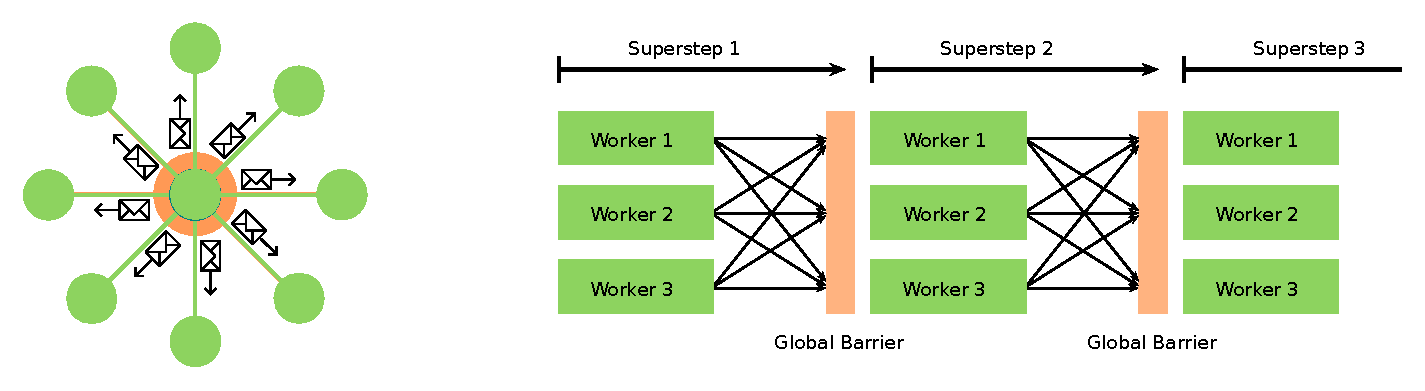
\includegraphics[
                        width = 0.8\paperwidth,
                        height = 0.8\paperheight,
                        keepaspectratio
                    ]{images/ArangoDBCustomPregel2020sendmessage.pdf}
                \end{center}
        \end{columns}
        \note[item]{
            {\color{blue}\textit{go to next slide}}
        }
    \end{frame}
    
    \begin{frame}{Clustering results}
        \begin{center}
            \vspace*{-0.1cm}
            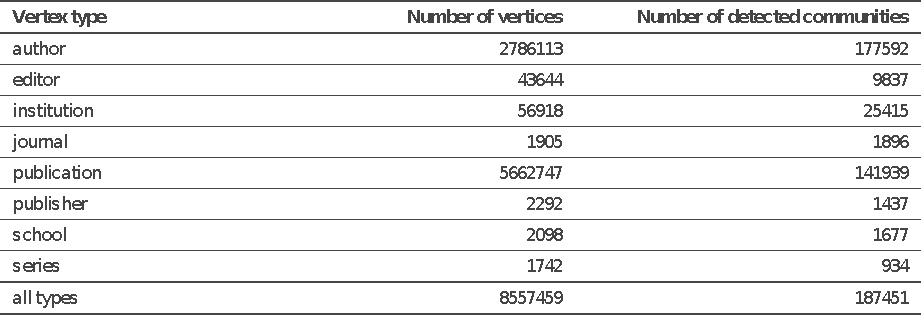
\includegraphics[
                width = 0.85\paperwidth,
                height = 0.85\paperheight,
                keepaspectratio
            ]{images/communitiesdetectedtable.pdf}
        \end{center}
        \note[item]{
            \begin{itemize}
                \item Nel grafo fatto da 8 milioni e mezzo di vertici e 24 milioni di archi,
                \item sono state individuate 187 milla communità.
            \end{itemize}
        }
        \note[item]{
            \begin{itemize}
                \item Mediamente in una community ci sono 
                \item 16 ricercatori, 2 instituti di affiliazione, 1 journal.
                \item Inoltre, generalmente i nodi di una community hanno fatto mediamente 40 pubblicazioni scientifiche e le pubblicazioni sono associate alla stessa scuola.
            \end{itemize}
            
        }
        \note[item]{
            \begin{itemize}
                \item Per vedere questi risultati in maniare visualmente apprezzabile,
                \item è stata sviluppata una Full-stack Web Application.
                \item Vediamo come è fatta:
            \end{itemize}
            
            {\color{blue}\textit{go to next slide}}
        }
    \end{frame}
    
    \begin{frame}{Web Application's Architecture}
        \begin{center}
            \vspace*{-0.1cm}
            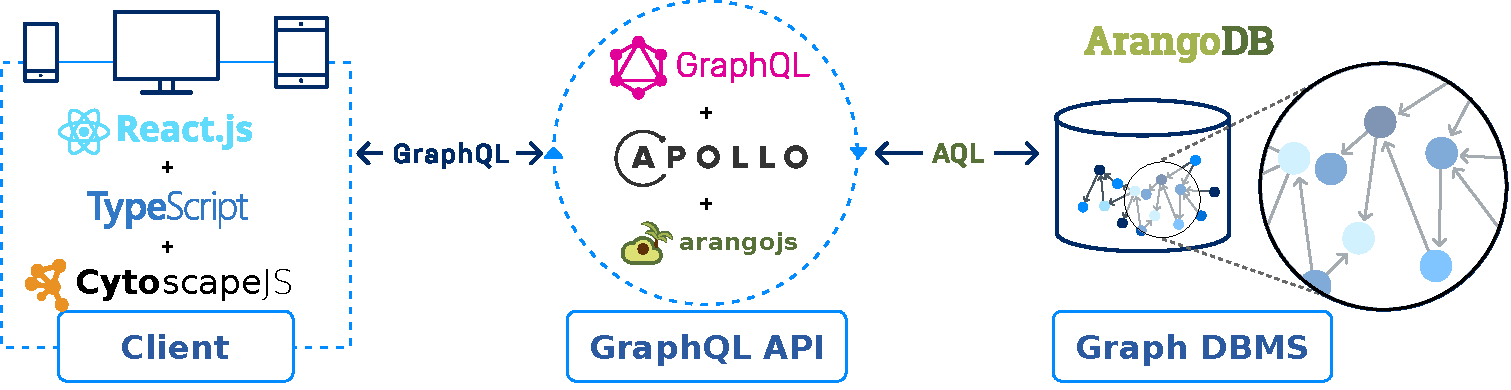
\includegraphics[
                width = 0.9\paperwidth,
                height = 0.9\paperheight,
                keepaspectratio
            ]{images/architecture.pdf}
        \end{center}
        \note[item]{
            {\color{blue}\textit{go to next slide}}
        }
    \end{frame}
    
    \begin{frame}{GraphQL API}
        \begin{center}
            \vspace*{-3cm}
            \hspace*{-0.3cm}
            
\includegraphics[
                width = 0.9\paperwidth,
                height = 0.9\paperheight,
                keepaspectratio
            ]{images/graphqlapollonew.pdf}
        \end{center}
        \note[item]{
            {\color{blue}\textit{go to next slide}}
        }
    \end{frame}
    
    \begin{frame}{Frontend UI Layout}
        \begin{center}
            \vspace*{-0.6cm}
            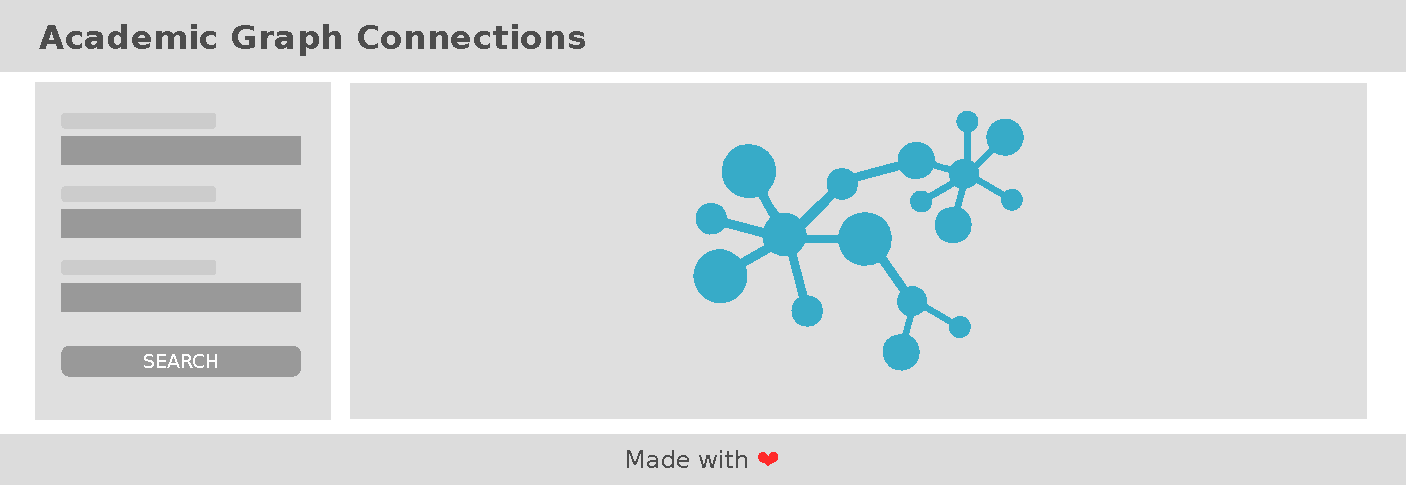
\includegraphics[
                width = 0.85\paperwidth,
                height = 0.85\paperheight,
                keepaspectratio
            ]{images/frontendlayout.pdf}
        \end{center}
        \note[item]{
            {\color{blue}\textit{go to next slide}}
        }
    \end{frame}
    
    \begin{frame}{Frontend UI Search Form}
        \begin{center}
            \vspace*{0.2cm}
            \hspace*{-1cm}
            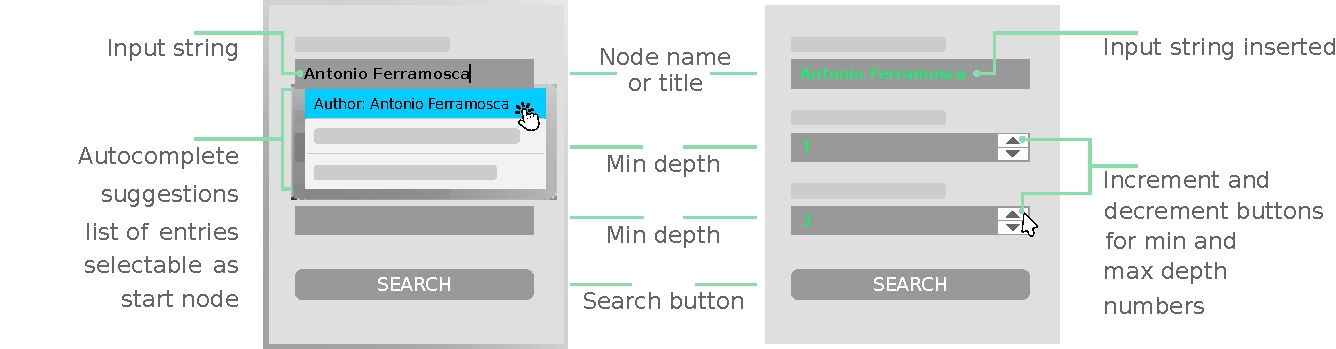
\includegraphics[
                width = 0.95\paperwidth,
                height = 0.95\paperheight,
                keepaspectratio
            ]{images/frontendsearchformautocompletenew.pdf}
        \end{center}
        \note[item]{
            \begin{itemize}
                \item \footnotesize La ricerca è implementata con una feature di autocompletamento
                \item \footnotesize in modo che l'utente possa selezionare un nodo dall'elenco dei nodi suggeriti
                \item \footnotesize e in background il suo nome o titolo verrà tradotto nel suo ID
                \item \footnotesize così poi da poterlo usare mentre si richiede il suo grafo delle collaborazioni.
            \end{itemize}
        }
        \note[item]{
            \begin{itemize}
                \item \footnotesize Nell'esempio mostrato in slide
                \item \footnotesize si è cercato il nodo rappresentante un autore di pubblicazioni scientifiche
                \item \footnotesize di nome "Antonio Ferramosca"
                {\color{orange}\textit{smile}}
            \end{itemize}
        }
        \note[item]{
            \begin{itemize}
                \item \footnotesize Gli altri due campi da compilare sono il minimum e il maximum depth.
                \item \footnotesize Essi rappresentano le distanze minime e massime che i nodi da visualizzare devono avere dal nodo di partenza.
            \end{itemize}
        }
        \note[item]{
            \begin{itemize}
                \item \footnotesize Vediamo un caso concreto.
                \item \footnotesize Ricerchiamo il grafo delle communità di collaborazione del professor Gargantini.
            \end{itemize}
            
            {\color{blue}\textit{go to next slide}}
        }
    \end{frame}
    
    \begin{frame}{Results display (Searching for "Angelo Gargantini")}
        \begin{center}
            \vspace*{-0.83cm}
            \hspace*{-1.06cm}
            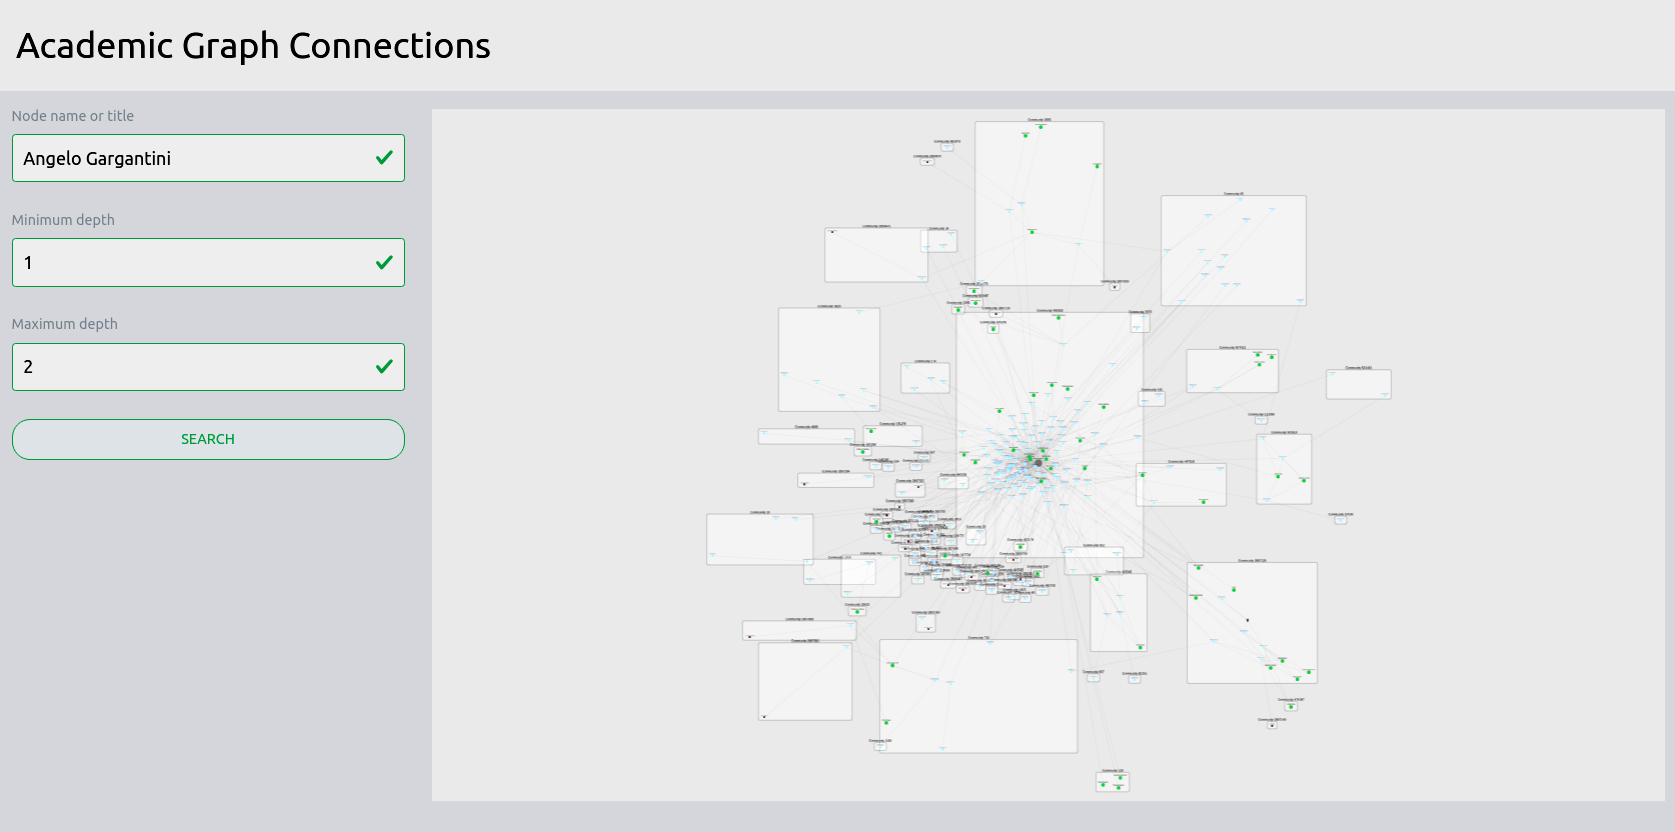
\includegraphics[
                width = 1\paperwidth,
                height = 1\paperheight,
                keepaspectratio
            ]{images/SnapshotLoadedGraphGargantininew.png}
        \end{center}
        \note[item]{
            {\color{blue}\textit{go to next slide}}
        }
    \end{frame}
    
    \begin{frame}{Results display (Angelo Gargantini)}
        \begin{center}
            \vspace*{-0.83cm}
            \hspace*{-1.06cm}
            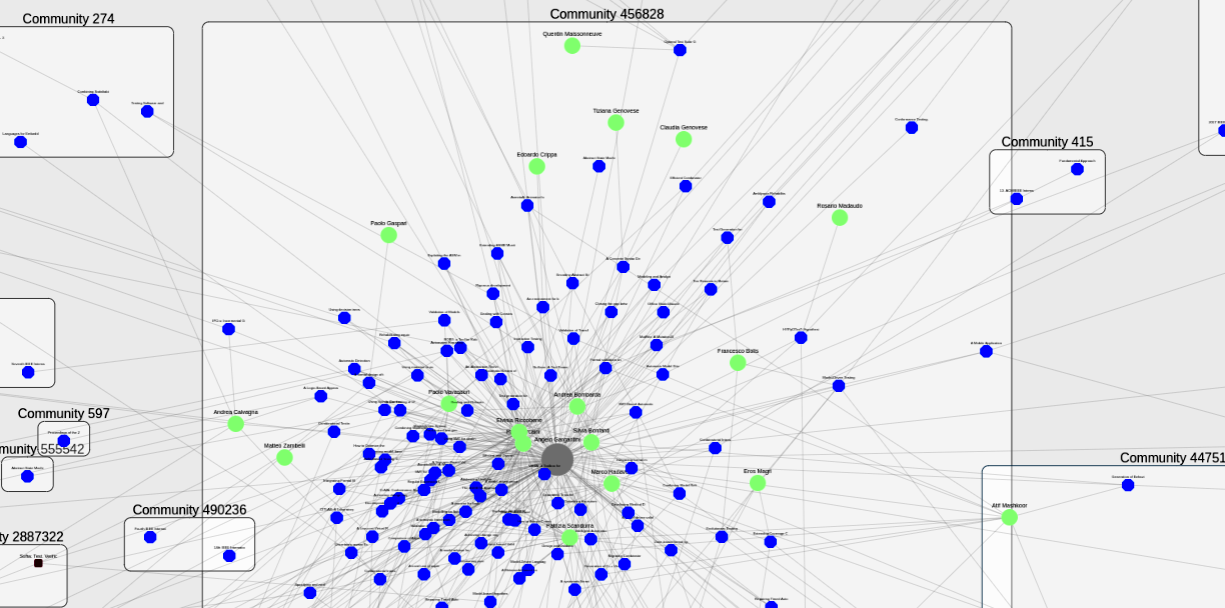
\includegraphics[
                width = 1\paperwidth,
                height = 1\paperheight,
                keepaspectratio
            ]{images/SnapshotLoadedGraphGargantiniZoomnew.png}
        \end{center}
        \note[item]{
            {\color{blue}\textit{go to next slide}}
        }
    \end{frame}
    
    \begin{frame}{}
        \begin{tikzpicture}[remember picture,overlay]
            \begin{pgfonlayer}{background}
                \node[anchor=south east,outer sep=0pt,inner sep=0pt] at ($(current page.south east) +(-0in,0in)$) {
                    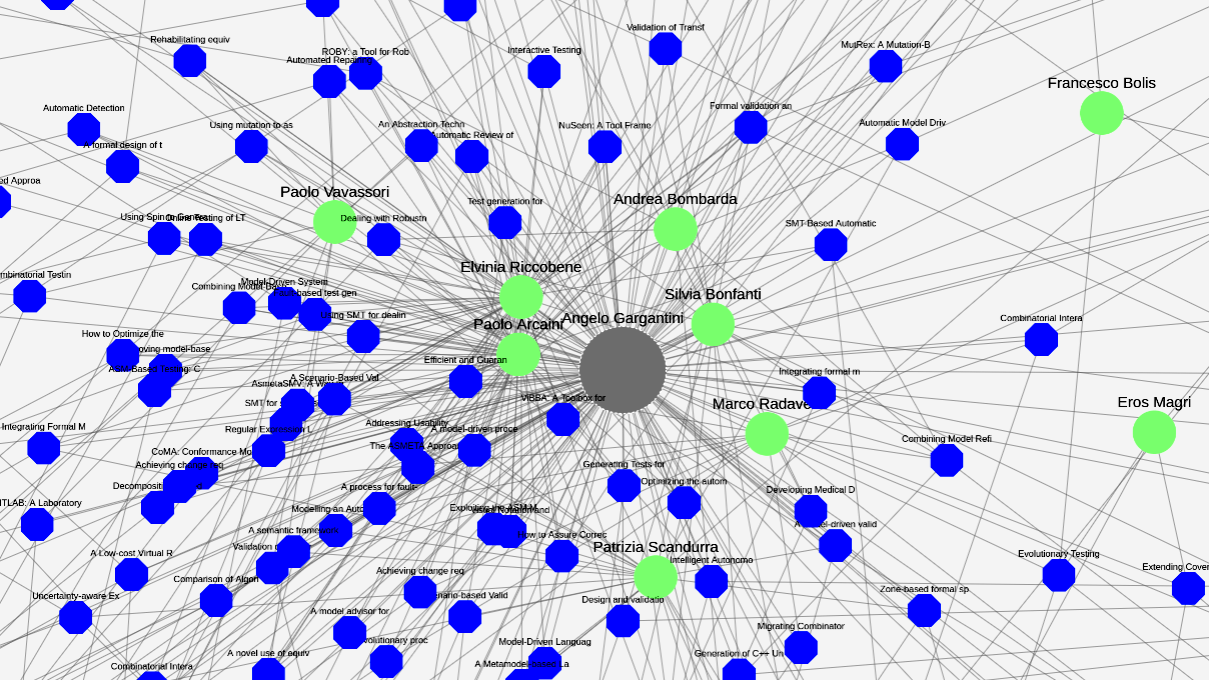
\includegraphics[
                        width = 1\paperwidth,
                        height = 1\paperheight,
                        keepaspectratio
                    ]{images/SnapshotLoadedGraphGargantiniZoomMorenew.png}
                };
            \end{pgfonlayer}
        \end{tikzpicture}
        \note[item]{
            {\color{blue}\textit{go to next slide}}
        }
    \end{frame}
    
    \begin{frame}{Results display (Patrizia Scandurra)}
        \begin{center}
            \vspace*{-0.83cm}
            \hspace*{-1.06cm}
            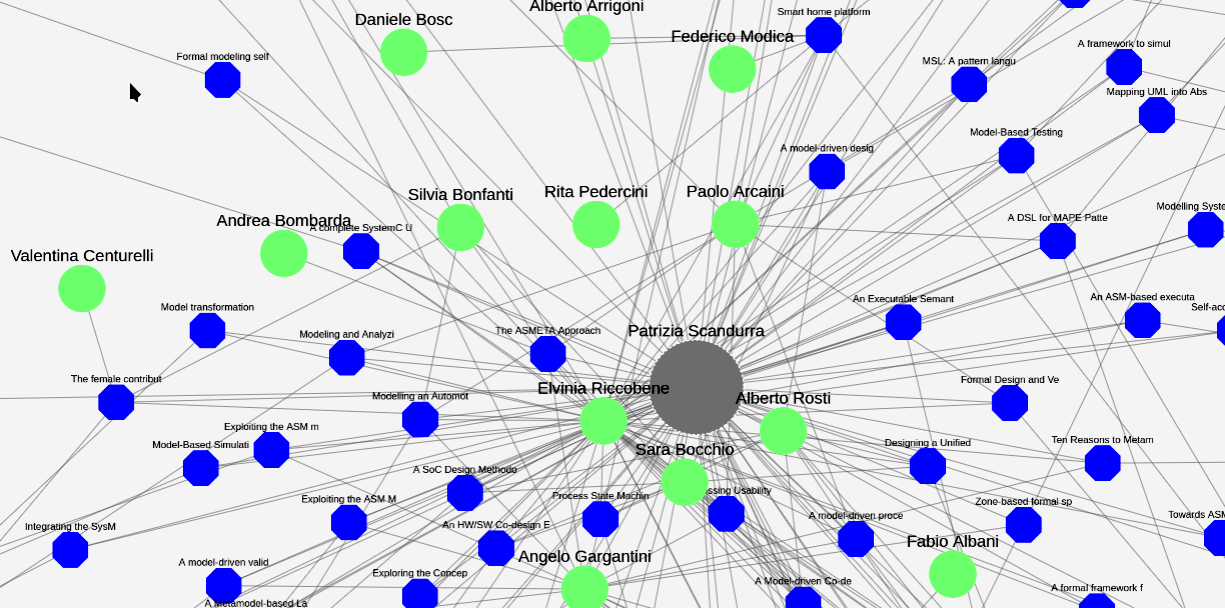
\includegraphics[
                width = 1\paperwidth,
                height = 1\paperheight,
                keepaspectratio
            ]{images/SnapshotLoadedGraphScandurraZoomMorenew.png}
        \end{center}
        \note[item]{
            {\color{blue}\textit{go to next slide}}
        }
    \end{frame}
    
    \begin{frame}{Results display (Giuseppe Psaila)}
        \begin{center}
            \vspace*{-0.83cm}
            \hspace*{-1.06cm}
            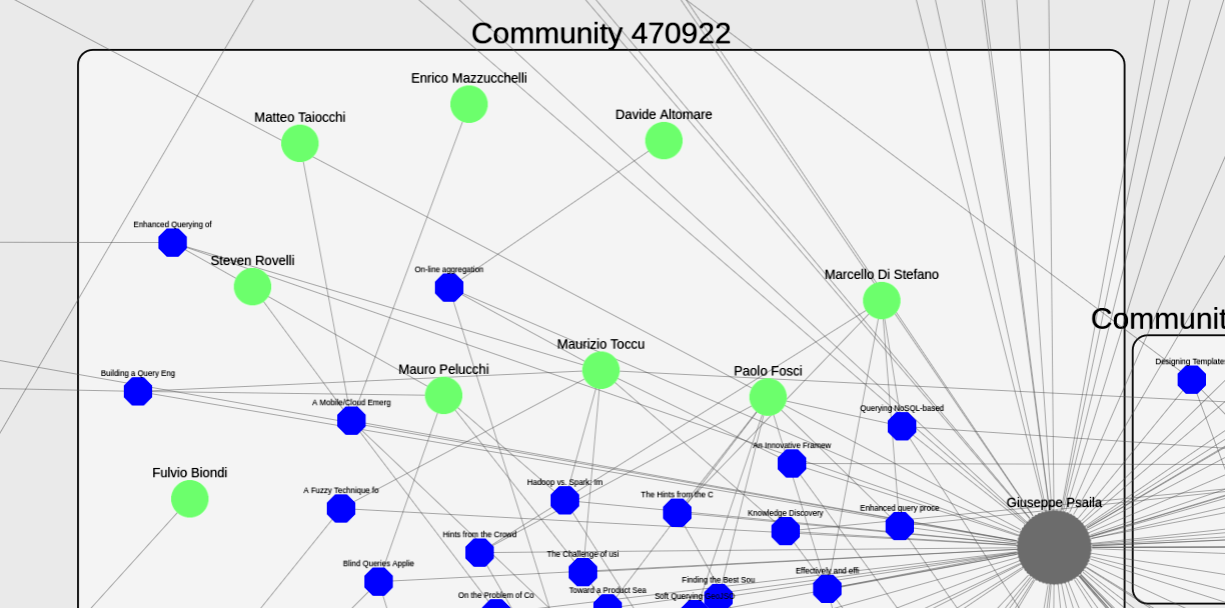
\includegraphics[
                width = 1\paperwidth,
                height = 1\paperheight,
                keepaspectratio
            ]{images/SnapshotLoadedGraphPsailaZoomMorenew.png}
        \end{center}
        \note[item]{
            In questa slide è mostrato zoomato il grafo delle communities di collaborazione del prof. Psaila.
        }
        \note[item]{
            È possibile riconoscere subito i suoi assistenti, Fosci e Pelucchi.
            
            {\color{blue}\textit{go to next slide}}
        }
        \note[item]{
            Nella successiva slide verrà mostrato il grafo delle communità di collaborazione accademica ora non più di un autore specifico ... 
            
            {\color{blue}\textit{go to next slide}}
        }
    \end{frame}
    
    \begin{frame}{Results display (Statistical Methods \& Applications Journal)}
        \begin{center}
            \vspace*{-0.83cm}
            \hspace*{-1.06cm}
            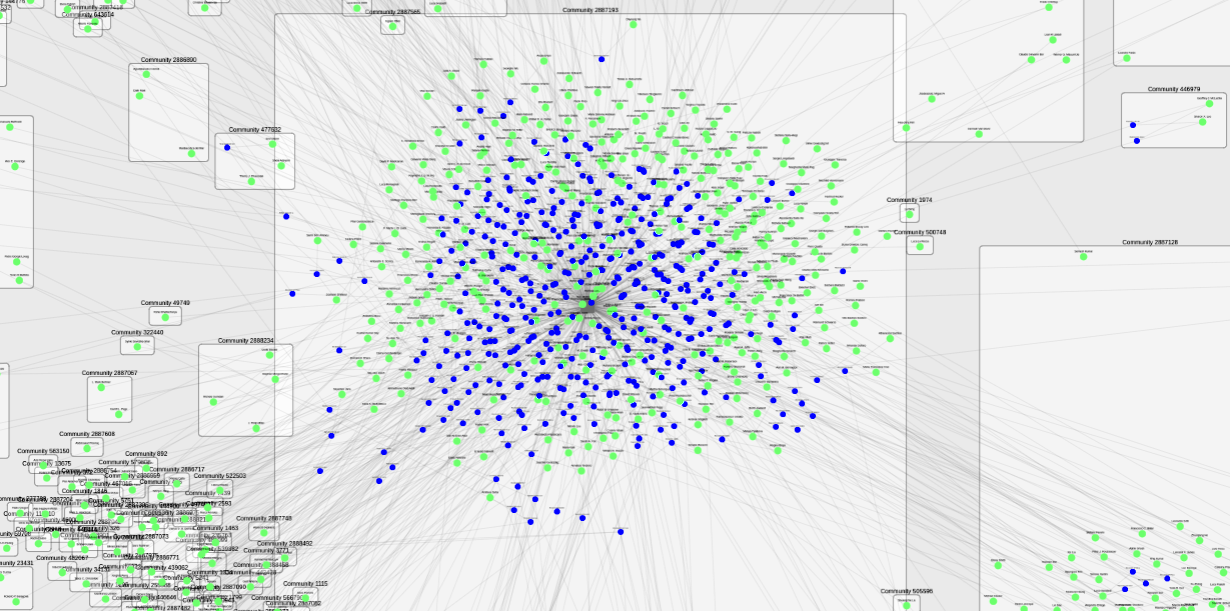
\includegraphics[
                width = 1\paperwidth,
                height = 1\paperheight,
                keepaspectratio
            ]{images/SnapshotLoadedGraphJournalZoomnew.png}
        \end{center}
        \note[item]{
            ... ma di un Journal come quello di Statistical Methods \& Applications.
            
            {\color{blue}\textit{go to next slide}}
        }
    \end{frame}
    
    \begin{frame}{Results display (ETH Zurich)}
        \begin{center}
            \vspace*{-0.83cm}
            \hspace*{-1.06cm}
            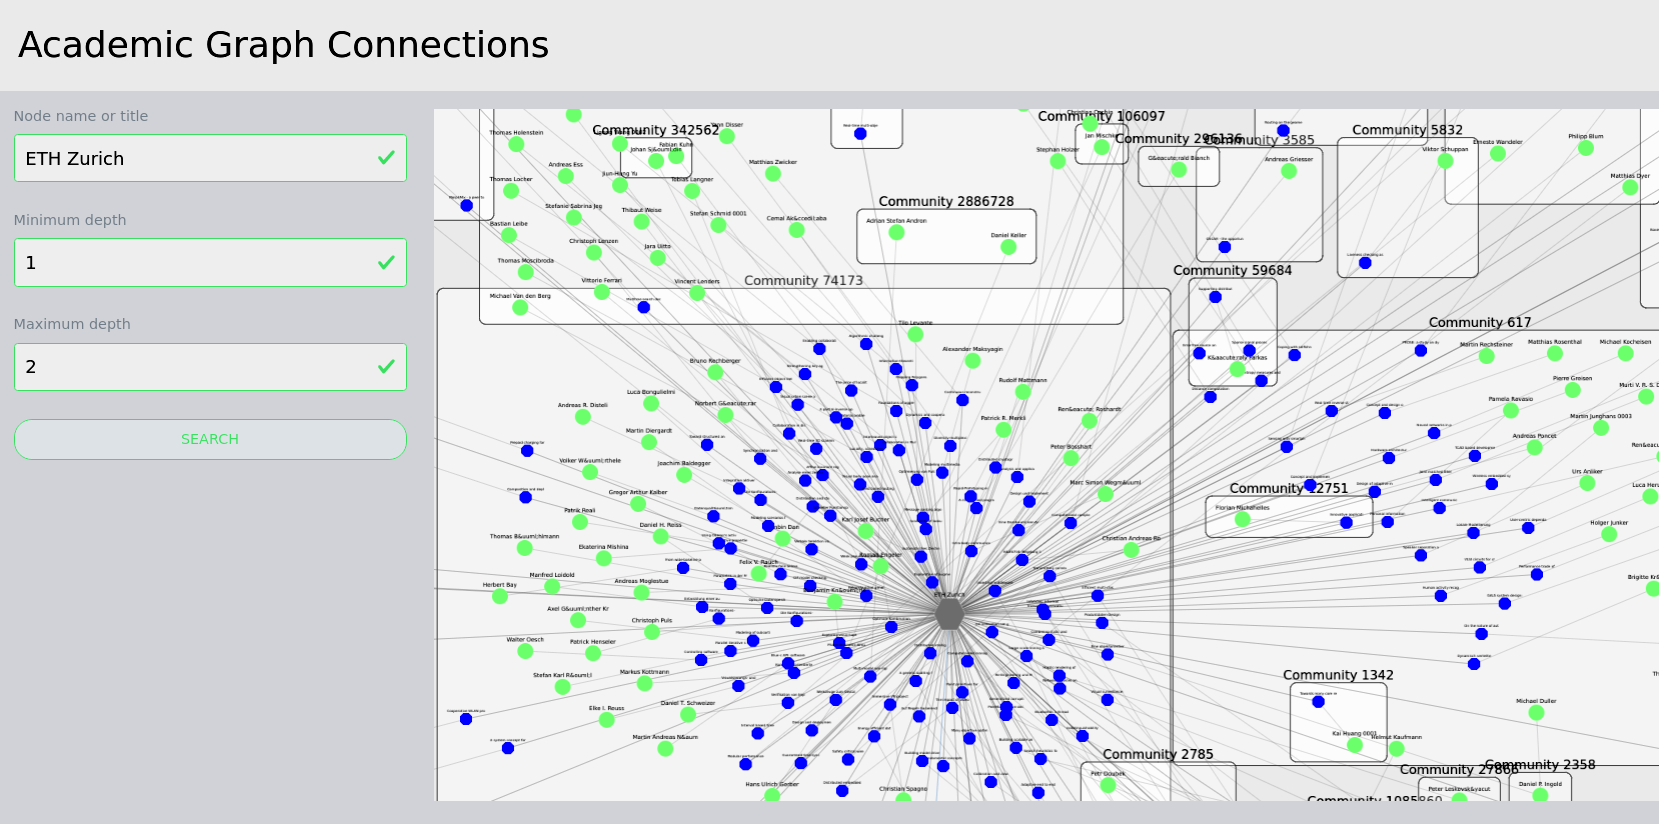
\includegraphics[
                width = 1\paperwidth,
                height = 1\paperheight,
                keepaspectratio
            ]{images/SnapshotLoadedGraphETHZurich12new.png}
        \end{center}
        \note[item]{
            {\color{blue}\textit{go to next slide}}
        }
    \end{frame}
    
    \begin{frame}[standout]
        \normalfont
        \vspace*{2.25cm}
        \Huge Thank you!
        
        \vspace*{0.625cm}
        Questions?
        
        \vspace*{0.125cm}
        \begin{columns}[t]
            \column{.08\textwidth}
            
            \column{.17\textwidth}
                \centering\normalsize\break\myauthor
                
            \column{.25\textwidth}
                \vspace*{-0.9cm}
                \begin{flushright}
                    \large\textbf{\textsc{\break\mydocumenttitle}}
                \end{flushright}
                
            \column{.315\textwidth} \scriptsize\normalfont\break\mydocumentsubtitle
                
            \column{.10\textwidth}
        \end{columns}
        \note[item]{
            \normalfont
            Grazie mille a tutti per l'attenzione!
        }
        \note[item]{
            \normalfont
            Se avete delle domande...
            
            {\color{orange}\textit{wait for questions}}
        }
    \end{frame}

\end{document}
